\documentclass{ieeeaccess}
% IEEE Access survey article. Template: ACCESS_latex_template_20260513 (official, ieeeaccess.cls),
% assets copied verbatim from ../../paper_beyond_exponential_decay/.
% Build: bash build.sh  (pandoc .md -> body.tex fragment; pdflatex -> bibtex -> pdflatex x2)
\usepackage{cite}
\usepackage{amsmath,amssymb,amsfonts}
\usepackage{graphicx}
\usepackage{textcomp}
\usepackage{booktabs}
\usepackage{array}
\usepackage{calc}
\usepackage{longtable}
\usepackage{tabularx}
\usepackage{url}
\usepackage{enumitem}
\setlist{nosep,leftmargin=*}
\graphicspath{{figures/}}
\usepackage[utf8]{inputenc}
\DeclareUnicodeCharacter{2265}{\ensuremath{\geq}}
\DeclareUnicodeCharacter{2264}{\ensuremath{\leq}}
\DeclareUnicodeCharacter{2192}{\ensuremath{\rightarrow}}
\DeclareUnicodeCharacter{2282}{\ensuremath{\subset}}
\DeclareUnicodeCharacter{2248}{\ensuremath{\approx}}
\DeclareUnicodeCharacter{00D7}{\ensuremath{\times}}
\DeclareUnicodeCharacter{2211}{\ensuremath{\sum}}
\DeclareUnicodeCharacter{221E}{\ensuremath{\infty}}
\DeclareUnicodeCharacter{03B5}{\ensuremath{\varepsilon}}
\DeclareUnicodeCharacter{03C4}{\ensuremath{\tau}}
\DeclareUnicodeCharacter{03BB}{\ensuremath{\lambda}}
\DeclareUnicodeCharacter{03A9}{\ensuremath{\Omega}}
\DeclareUnicodeCharacter{03B8}{\ensuremath{\theta}}
\DeclareUnicodeCharacter{2013}{--}
\DeclareUnicodeCharacter{2014}{---}

% float placement: let several two-column tables sit at the top of one page instead of queuing to the end
\setcounter{dbltopnumber}{3}
\setcounter{topnumber}{3}
\setcounter{totalnumber}{5}
\renewcommand{\dbltopfraction}{0.95}
\renewcommand{\topfraction}{0.95}
\renewcommand{\textfraction}{0.05}
\renewcommand{\dblfloatpagefraction}{0.6}
\renewcommand{\floatpagefraction}{0.6}
\renewcommand{\textfraction}{0.05}

% pandoc fragment support
\providecommand{\tightlist}{\setlength{\itemsep}{0pt}\setlength{\parskip}{0pt}}
\newcounter{none}  % absorbs pandoc longtable caption counters
\makeatletter
\providecommand{\pandocbounded}[1]{#1}
\makeatother

\begin{document}
\history{Date of publication xxxx 00, 0000, date of current version xxxx 00, 0000.}
\doi{10.1109/ACCESS.2026.0000000}

\title{Frontier and Localhost: A Survey of How Production AI Learns Outside the Weights}

% TODO(authors): confirm city/country for each address, middle initials, ORCIDs, and IEEE membership if any.
\author{\uppercase{Mikhail L. Arbuzov}\authorrefmark{1},
\uppercase{Lee Mosbacker}\authorrefmark{2},
\uppercase{Sisong Bei}\authorrefmark{3},
\uppercase{Ziwei Dong}\authorrefmark{4},
\uppercase{Dmitri Kalaev}\authorrefmark{5},
AND \uppercase{Alexey Shvets}\authorrefmark{6}}

\address[1]{Independent Researcher, CITY, COUNTRY (e-mail: mike.arbuzov54@gmail.com)}
\address[2]{Independent Researcher, CITY, COUNTRY (e-mail: lee.mosbacker@gmail.com)}
\address[3]{Independent Researcher, CITY, COUNTRY (e-mail: qurining@gmail.com)}
\address[4]{Independent Researcher, CITY, COUNTRY (e-mail: ziwei.dong@alumni.emory.edu)}
\address[5]{Independent Researcher, CITY, COUNTRY (e-mail: kalaevdr@gmail.com)}
\address[6]{Palo Alto Networks, CITY, COUNTRY (e-mail: ashvets@paloaltonetworks.com)}
\tfootnote{TODO(authors): funding statement, e.g., ``This work received no external funding.'' A. Shvets is employed by Palo Alto Networks; the views expressed are the authors' own.}

\markboth
{Arbuzov \headeretal: Frontier and Localhost}
{Arbuzov \headeretal: Frontier and Localhost}

\corresp{Corresponding author: Mikhail L. Arbuzov (e-mail: mike.arbuzov54@gmail.com).}

\begin{abstract}
Deployed AI systems change through instructions, skills, memories, tools, and orchestration long before their model weights are updated. These edits accumulate experience, but their persistence alone does not establish that the system is improving. This survey examines how 256 production and research systems turn experience into lasting edits outside the weights. We distinguish two decisions: whether an edit improves the deployment that produced it, and whether enough evidence supports sharing it more widely. These decisions define a local improvement loop and a promotion loop. The feedback these loops receive (exact checks, observed outcomes, judgments, or delayed outcomes) supports different acceptance rules and exposes different limitations. In every case, an accepted edit is supported only for the measure and tasks on which it was evaluated. We use this observation to develop five conditions for artifact-layer optimization, a classification of feedback and gate types, and four properties for auditing promotion across organizations. The resulting framework identifies what existing systems can already automate and where new evidence or human judgment is still required. Nearly every recently added system with a local loop has an automatic acceptance test (89 of 96), while failure records and credit assignment remain less developed. Promotion is more fragmented: the surveyed systems provide evaluation, shared artifact pools, lineage, access control, and rollback in different combinations, but none documents their integration into governed promotion across organizations. The feedback available to a deployment helps explain this pattern.

\end{abstract}

\begin{keywords}
AI governance, agent memory, agent skills, evaluation, large language models, LLM agents, prompt optimization, self-improving systems, survey
\end{keywords}

\titlepgskip=-21pt

\maketitle

\section{Introduction}\label{sec:intro}

In one repository, a coding agent repeatedly uses the wrong naming convention. An engineer adds a line to the agent's instructions, and the next session follows the convention. The model has not changed, but the deployed system has. The same happens when an assistant corrects a stored preference, acquires a reusable skill, or learns which tool to call. Persistent artifacts like these, outside the model's weights, now accumulate much of the experience that makes an AI system useful in one setting.

We call this layer the \textbf{scaffold}. It includes instructions, skills, memory, tools, orchestration, and the evaluation and governance rules that control their use. In the language of compound AI systems \cite{zaharia2024compound}, it is the part surrounding the model that a deployment can inspect and revise without retraining. The split matters because the two change on different schedules: a team can revise an instruction or tool binding as soon as a problem is understood, while a new model must go through separate training, evaluation, and release.

But because edits are easy to make, edits of unknown value are easy to accumulate. A rule added after one incident may prevent a recurring error, conflict with another rule, or merely make the prompt longer. A memory may be corrected in the history while the system keeps retrieving the outdated entry. Even a demonstrably useful edit can become harmful when copied into a deployment with different tasks or conventions. Researchers pay a different cost: without knowing whether a system tests its edits, they cannot tell whether a system described as self-improving improved anything, cannot compare two such systems, and may build on a loop with no acceptance test or no failure record.

These situations leave two questions unanswered: what evidence justifies keeping a local edit, and what additional evidence justifies sharing it? The first defines a \textbf{local loop}: identify a recurring failure, propose an edit to the responsible artifact, and test whether it helps. The second defines a \textbf{promotion loop}: decide whether another project, team, or organization should adopt the edit, and preserve enough history to reverse that decision. This survey uses those questions to examine 256 public production and research systems.

The surveyed systems have built these loops unevenly. Nearly every recently added system with a local loop has an automatic acceptance test: 89 of 96. The steps that should supply those tests with well-founded candidates are weaker: failures are often not retained in a usable form, and a failed output rarely identifies the instruction, memory, skill, or tool binding at fault. Production platforms, by contrast, have built substantial versioning and release machinery but no process that proposes edits from deployment experience.

Promotion is more fragmented. No surveyed system documents an automatic local loop connected to promotion across organizations, with versioned lineage, access control, and rollback. Shared formats and registries make artifacts portable, but they do not establish that an artifact will help its recipient. Some surveyed systems check transferred edits within one operator.

Feedback differs across systems and supports different kinds of automation. A compiler or test suite can check a candidate immediately. A booked appointment is a later, noisier outcome. A writing task may depend on a judge whose preferences can drift. A research decision may take months to evaluate. In the surveyed systems, then, the local gate is built nearly everywhere a local loop exists, the failure record and credit assignment that feed it are weaker, and governed promotion across organizations is unassembled. Feedback helps explain this pattern, and no feedback establishes an improvement beyond what it measures.

The survey develops a framework for reading its evidence, which consists of published methods and public documentation; it introduces no new experiments, and its scores and classifications are released for inspection. We define the two loops and when maintaining artifacts counts as optimization, then describe the corpus and scoring method and examine the local loop, the feedback that constrains it, and the evidence needed for promotion. The later sections consider failures that arise without gates, specify the unassembled architecture for governed promotion, and connect the findings to the research lines that produced its components.

\section{From a local fix to a measured improvement}\label{sec:loop}

Adding a naming rule after an error is reasonable, but the team learns whether it works only by rerunning the agent on relevant tasks and comparing results. If the edit helps, it should persist; if it causes regressions, the team needs a way to reject or reverse it. Repeating this process turns a growing collection of fixes into a procedure for improving the deployment.

\subsection{The local loop}\label{the-local-loop}

The procedure starts with a record of failures: rejected answers, user corrections, failed tool calls, evaluation regressions, or unsuccessful tasks. Repeated failures are grouped into modes and prioritized by frequency and severity. For each selected mode, the system tries to identify the artifact responsible. A stale memory entry needs a different fix from a missing tool argument or an ambiguous instruction.

We call this step \textbf{credit assignment}. It links an observed failure to an editable part of the scaffold: a \textbf{coordinate}. The system then proposes a candidate edit and evaluates it against the current scaffold. The acceptance test is the \textbf{gate}. An accepted edit is retained as a versioned artifact; a later regression can trigger rollback. Fig.~\ref{fig:descent} shows the complete local loop.

\begin{figure*}[!t]
\centering
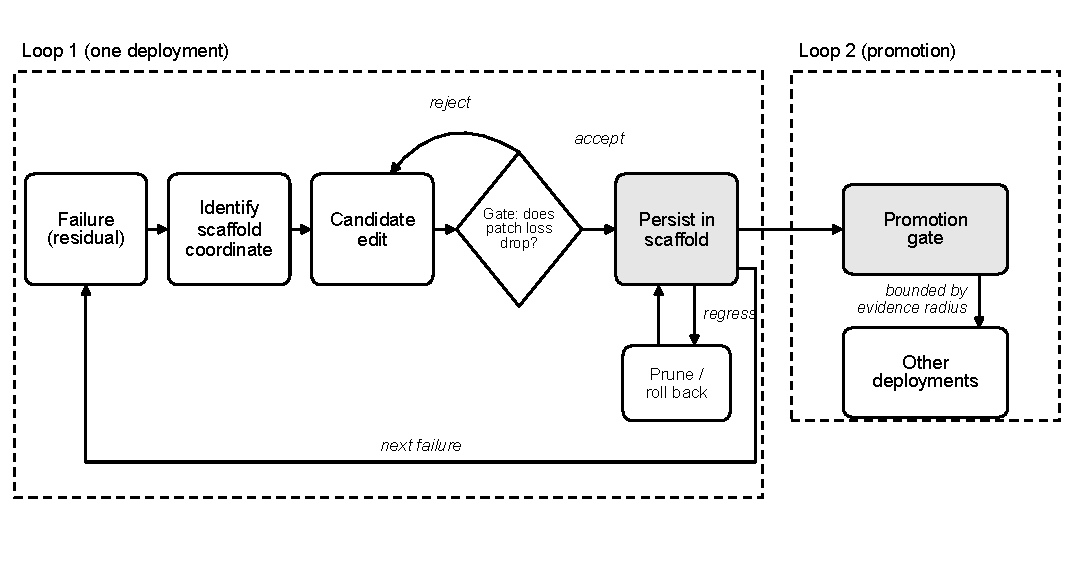
\includegraphics[width=\textwidth]{fig1_descent_ieee}
\caption{The local improvement loop. Recurring failures guide a proposed scaffold edit. An acceptance gate tests the change before it persists, and later regressions can trigger rollback. Sharing the accepted edit requires a separate promotion decision (Fig.~\ref{fig:scope}).}
\label{fig:descent}
\end{figure*}

The gate's evaluation must be tied to the deployment's workload. A deployment serves a distribution of users, tasks, and conventions, which we call its \textbf{patch}. Its \textbf{patch loss} measures failure on that distribution. Depending on the application, the patch loss may be a task-failure rate, correction rate, retrieval error, or another operational measure. A gate can establish an improvement only as far as its evaluation estimates the patch loss.

\subsection{The second decision: whether to share the fix}\label{the-second-decision-whether-to-share-the-fix}

Suppose the naming rule helps in the original repository and the team considers adding it to a shared template. That decision changes the population the rule will act on. Other repositories may follow a different convention, about which the local evaluation says little.

The promotion loop therefore asks for evidence at the receiving scope. We call this \textbf{receiving-side evaluation}: a check on the tasks of the deployment that would adopt the edit. The scope for which the available evaluation supports an edit is its \textbf{evidence radius}, and a local success does not automatically enlarge that radius. Section~\ref{sec:design} develops the scopes and examines systems that transfer artifacts between them.

\subsection{Five conditions for artifact-layer optimization}\label{five-conditions-for-artifact-layer-optimization}

We use \textbf{artifact-layer descent} for maintenance that connects recurring failures to measured improvements by meeting five conditions:

\begin{enumerate}
\def\labelenumi{\arabic{enumi}.}
\tightlist
\item
  \textbf{A measurable patch loss:} the deployment has a defined measure of success or failure.
\item
  \textbf{A failure log:} relevant failures are retained as evidence for later edits.
\item
  \textbf{Credit assignment:} failures can, at least sometimes, be traced to the scaffold coordinates responsible.
\item
  \textbf{A candidate edit:} a process proposes an edit to those coordinates.
\item
  \textbf{An acceptance gate:} an edit is retained or promoted only after a check tests whether it lowers the relevant loss.
\end{enumerate}

These conditions distinguish three recurring forms of maintenance. In \emph{patchwork}, an engineer adds a rule after an incident without measuring the result. In \emph{random artifact search}, a system tests many variants and keeps a winner without tracing failures to their causes. In artifact-layer descent, the trace from failure to cause directs the proposed edit, which is tested before acceptance. Where the conditions are only partly met, the optimization interpretation is correspondingly limited.

For deployment \(D\), with edits that outlast the current interaction, write the patch loss as \[L_D(\theta_s)=\mathbb{E}_{x\sim D}\!\left[\ell(\pi(\theta_M,\theta_s,x))\right],\] where \(\theta_M\) denotes the fixed model weights, \(\theta_s\) the editable scaffold, and \(\ell\) the operational loss. A proposal process uses the failure history to produce an edit \(z_t\). There is no analytic gradient through an instruction file or memory entry.

Instead, the gate estimates the change in loss and accepts the edit when that estimate clears a required margin: \[G_t(z_t)=1\iff\widehat{\Delta}_{z_t}L_D(\theta_s^t)+\lambda\Omega(z_t)\leq-\tau_t.\] Here \(\Omega\geq0\) penalizes edit complexity and promotion breadth, and \(\tau_t\geq0\) is the acceptance margin. An evaluation that blocks a regressing merge applies this rule in practice. A reviewer or governance process can also instantiate the gate by requiring stronger evidence for a broader or more complex edit.

Appendix~\ref{app:formal} gives the update rule and a one-step descent inequality under assumptions on the gate's estimation bias. Improving edits eventually stop clearing the gate under additional coverage, compactness, and summable-bias assumptions. This is \textbf{gate stability}, not a claim of global optimality. A limited proposal process or biased evaluator can leave useful edits undiscovered or rejected.

\subsection{Who proposes and who decides}\label{who-proposes-and-who-decides}

Who writes an edit and who accepts it are separate roles. An agent may draft an edit that a person approves; an engineer may write an edit that an automatic evaluation rejects. We classify the gate by who decides whether to accept the edit:

\begin{itemize}
\tightlist
\item
  \textbf{Auto:} a program applies a check, including a verifier, evaluation threshold, or language-model judge \cite{zheng2023judge}. Section~\ref{sec:signal} asks separately whether that judge has been calibrated against people.
\item
  \textbf{Human:} a person decides whether to accept the edit.
\item
  \textbf{None:} nothing accepts or rejects the edit, either because the loop is absent or because every proposed edit is retained.
\end{itemize}

A pair such as {[}Auto × Human{]} denotes an automatic local gate followed by a human promotion gate. These labels describe the decision mechanism; by themselves, they do not establish that the decision is well supported.

From the loss definition, every loop inherits two limits. First, an accepted edit is evidence of improvement only on the measure and tasks evaluated. Promotion must preserve that scope or establish the improvement again. Second, the loop optimizes a defined objective. Revising the evaluator changes the objective itself, a complication we return to in Section~\ref{sec:reflexive}, but the loop does not discover a better objective simply by accumulating edits.

\section{Corpus and method}\label{sec:method}

We read each system's public method or documentation for four things: the persistent artifact the system changes, the feedback that prompts a change, the decision that accepts the change, and the scope in which the result is used. We then compare systems with different names and application domains by their behavior.

\subsection{Scope and selection}\label{scope-and-selection}

The corpus contains 256 unique systems from January 2023 through the October 2026 cutoff. The first search pass identified 130 systems by May 2026; the second added 126. Sources include research papers, public repositories, product documentation, and supported production reports. The released data (Supplementary Material S2) record the search families, evidence tiers, and inclusion rules.

A system enters the survey if it adapts a foundation model through a persistent artifact updated from deployment signal, or if it is publicly described as self-improving, scaffolded, or agentic. The second group forms a contrast set, with which the survey can test whether those descriptions correspond to persistent adaptation. We exclude systems whose only update mechanism is weight-level training, and systems without public evidence of release or deployment.

We apply two filters. Under the rubric below, the first admits a system to the \textbf{core corpus} if it scores at least 3 on at least one scaffold substrate. Of the 256 systems, 204 form the core corpus and 52 the contrast corpus. These 256 systems occupy 269 scored rows, because a system may have one integrated row or several substrate-specific rows.

The second filter is a \textbf{two-loop audit}. It asks whether session feedback changes a persistent artifact and whether that artifact is then promoted, with versioning or lineage, beyond the deployment that produced it. The audit covers 202 of the 204 core systems and 4 research systems classified from their papers alone (SkillOpt, FederatedSkill, SkillClaw, and ChronoMem); it admits 11 research systems and 3 industry exemplars. The eight systems without an audit are listed with the contrast set (Supplementary Material S4). Fig.~\ref{fig:corpus} summarizes the selection.

\begin{figure}[!t]
\centering
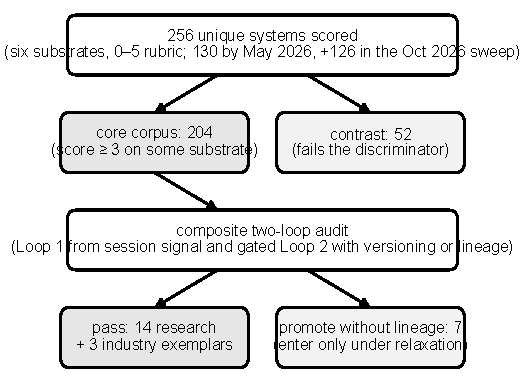
\includegraphics[width=\columnwidth]{fig4_corpus_flow_ieee}
\caption{Corpus selection. The 256 systems occupy 269 scored rows. The first filter separates core from contrast systems; the two-loop audit then checks persistent local adaptation and promotion with lineage. The audit includes the additional paper-based classifications described in the text.}
\label{fig:corpus}
\end{figure}

The research systems passing the audit are NanoResearch, SkillOpt, AlphaEvolve, ADAS, DGM, Voyager, SAGE, EvolveR, CoEvoSkills, AutoManual, and CASCADE. The industry exemplars are Sierra Agent OS 2.0, Cognition Devin, and Letta's Context Repositories. SkillOpt is not a row in the 256-system score table. The remaining paper-based systems are identified in the data notes (Supplementary Material S2), and the audit's boundary cases are identified in the contrast set (Supplementary Material S4).

Passing this audit does not establish governed sharing across organizations. All passing systems promote within one operator, into a shared bank or archive that later runs draw from, or across the agents and sessions of one deployment. Letta passes on the lineage of its shared-memory updates even though those updates have no acceptance gate. Six further systems promote across contexts without lineage on the promoted artifact; we report their treatment under relaxed audit rules separately.

\subsection{Substrates and scoring}\label{substrates-and-scoring}

The scaffold has six substrates: instructions, skills, memory, tools, orchestration, and governance. These are the possible targets of a proposed edit. Table~\ref{tab:V-1} describes them. Following Sumers et al. \cite{sumers2023coala}, we divide memory into episodic, semantic, and procedural categories.

\begin{table*}[!t]
\caption{The six scaffold substrates, what each holds, and what a system must do on it to score 5.}\label{tab:V-1}
\centering\small
\begin{tabular}{@{}
  >{\raggedright\arraybackslash}p{(\textwidth - 4\tabcolsep) * \real{0.1642}}
  >{\raggedright\arraybackslash}p{(\textwidth - 4\tabcolsep) * \real{0.4179}}
  >{\raggedright\arraybackslash}p{(\textwidth - 4\tabcolsep) * \real{0.4179}}@{}}
\toprule\noalign{}
\begin{minipage}[b]{\linewidth}\raggedright
Substrate
\end{minipage} & \begin{minipage}[b]{\linewidth}\raggedright
What persists
\end{minipage} & \begin{minipage}[b]{\linewidth}\raggedright
A score of 5 requires
\end{minipage} \\
\midrule\noalign{}


S1 Instructions & Project, team, or organization rules attached to a workspace & Versioned rules promoted under an automatic gate \\ \addlinespace[2.5pt]
S2 Skills & Procedures, as code or text, loaded on demand & A skill bank that edits itself on failure, test-gated, versioned, and promoted \\ \addlinespace[2.5pt]
S3 Memory & Experience kept across sessions: episodic, semantic, procedural & Provenance, versions, and a correction path for every entry \\ \addlinespace[2.5pt]
S4 Tools & The vetted action surface and its schemas & Evaluation-gated tool versions; a curated bundle as the product \\ \addlinespace[2.5pt]
S5 Orchestration & The multi-role graph and its routing & Topology updated from deployment feedback by a loop outside the agent's own run \\ \addlinespace[2.5pt]
S6 Governance & Versioning, promotion, audit, rollback & Staged promotion with evaluation thresholds, an audit log, and rollback \\ \addlinespace[2.5pt]
\bottomrule\noalign{}
\end{tabular}
\end{table*}
The shared scoring scale runs from 0 to 5. At 0 an artifact is ephemeral. At 1 it persists locally; at 2 it persists with tool attachment but without feedback. At 3 it either spans scopes without a gate or is updated from feedback by a person. At 4 a program updates it from feedback. The table's last column gives a separate score-5 requirement for each substrate.

A score of 5 thus certifies different things on different substrates. On instructions and skills it requires both loops; on orchestration, a topology updated from deployment feedback by a loop outside the agent's own execution. On memory, tools, and governance it measures the corresponding governance capability, so a registry can score 5 without generating local edits. On integrated rows it measures breadth and depth of adaptation, not closure of either loop. The scale therefore supports substrate-specific comparisons; no top score is a universal certificate of complete optimization.

In the corpus distribution (Table~\ref{tab:V-2}), research systems hold the top marks on skills, memory, and the integrated row, and production platforms hold them on governance. No system reaches the top score across all six substrates, and none reaches it on instructions, tools, or orchestration.

\begin{table*}[!t]
\caption{Substrate maturity across the 256-system corpus. Column n counts scored rows on each substrate, Mean is the average score, and Score-5 systems reach the substrate's top mark; the integrated row counts systems scored across several substrates as one row. Of the 126 most recently added systems, 105 are core and 32 are skill systems; 96 of those core systems have a local loop and 89 close it under a program, and none of the 126 scores 5 on any substrate.}\label{tab:V-2}
\centering\small
\begin{tabular}{@{}
  >{\raggedright\arraybackslash}p{(\textwidth - 8\tabcolsep) * \real{0.1600}}
  >{\raggedleft\arraybackslash}p{(\textwidth - 8\tabcolsep) * \real{0.0533}}
  >{\raggedleft\arraybackslash}p{(\textwidth - 8\tabcolsep) * \real{0.0667}}
  >{\raggedright\arraybackslash}p{(\textwidth - 8\tabcolsep) * \real{0.2667}}
  >{\raggedright\arraybackslash}p{(\textwidth - 8\tabcolsep) * \real{0.4533}}@{}}
\toprule\noalign{}
\begin{minipage}[b]{\linewidth}\raggedright
Substrate
\end{minipage} & \begin{minipage}[b]{\linewidth}\raggedleft
\(n\)
\end{minipage} & \begin{minipage}[b]{\linewidth}\raggedleft
Mean
\end{minipage} & \begin{minipage}[b]{\linewidth}\raggedright
Score-5 systems
\end{minipage} & \begin{minipage}[b]{\linewidth}\raggedright
What the corpus holds on it
\end{minipage} \\
\midrule\noalign{}


S1 Instructions & 15 & 3.07 & (none) & Rules persist across IDEs and agents and nothing measures them; no system closes both loops; ceiling 4 \\ \addlinespace[2.5pt]
S2 Skills & 50 & 3.34 & SAGE, COSPLAY & The local loop closes under a program in the research systems; the production repositories merge by hand \\ \addlinespace[2.5pt]
S3 Memory & 50 & 3.06 & Cuadros et al. & The ledger ships in products; the correction a gate would enforce is absent \\ \addlinespace[2.5pt]
S4 Tools & 20 & 3.35 & (none) & Production tools are widely shared; registries govern admission, not evaluation \\ \addlinespace[2.5pt]
S5 Orchestration & 37 & 3.08 & (none) & Topologies change under an evaluation gate; one structurally gated instance; no two-loop system with lineage \\ \addlinespace[2.5pt]
S6 Governance & 45 & 2.98 & Braintrust, Vellum, LangSmith Hub & Prompts-as-code mature; registries add lineage and rollback; no local loop generates a candidate \\ \addlinespace[2.5pt]
Integrated & 52 & 3.81 & NanoResearch, AutoAgent, SkillRL & Breadth and depth of adaptation, not the loop; reached only by research systems without enterprise governance \\ \addlinespace[2.5pt]
\bottomrule\noalign{}
\end{tabular}
\end{table*}
The rows of the 126 most recently added systems record gate types, feedback classes, and governance properties as explicit columns of the released table, and counts of these properties describe that subset alone. Of its 105 core systems, for example, 96 have a local loop and 89 close it under a program, a count that does not extend to all 256 systems.

\subsection{Evidence and limitations}\label{evidence-and-limitations}

The evidence ranges from peer-reviewed studies and open-source artifacts to vendor claims. Peer-reviewed papers and open-source artifacts receive the greatest weight. A production claim must name a benchmark or integration target, and a blog or interview counts only when corroborated by stronger evidence. Corpus-level statistics do not pool production claims with peer-reviewed evidence, and vendor-based exemplars are identified as such. Every row of the released table carries its source and a one-line justification, and the rows for the 126 most recently added systems also carry an evidence tier.

One author scored all systems. Ambiguous cases were rounded down, and half-scores were used only when one criterion was clearly met and another partly met. Independent re-rating remains future work. The classifications should be read as an auditable interpretation of public evidence, not a complete inventory of private production behavior.

We also test the audit under alternative boundaries: counting rollback as sufficient promotion governance, allowing promotion without governance, and admitting loops that persist only optimizer state. Membership changes under these relaxations, but the main structural findings hold: {[}Auto × Auto{]} stays well populated, the cells with a human local gate hold only curation and registries, Letta alone passes with an ungated promotion, and no relaxation adds governed promotion across organizations (Section~\ref{sec:gap}). The sensitivity analysis is released with the data notes (Supplementary Material S2) and the full score table with the released table (Supplementary Material S1).

\section{What local adaptation actually closes}\label{sec:findings}

A system can detect a failure, explain it, and write a plausible correction without ever establishing that the correction helps. SkillForge is such a system. Its judge agrees with people more than nine times in ten and identifies replies that should be rewritten. SkillForge updates the skill from those replies but commits the updated skill without an acceptance test \cite{skillforge2026}. The judge's calibration concerns which replies are inadequate; it does not measure the effect of the resulting skill edits.

SkillRL leaves its corrections untested by a different route. A success-rate threshold triggers proposals for new skills, and the skill bank accepts each proposal unconditionally \cite{skillrl2026}. Both systems respond to experience, yet neither has the local gate defined in Section~\ref{sec:loop}. Proposing an edit is not accepting it, so the survey records who accepts an edit separately from the edit's author and its trigger.

Among recent systems with a local loop, however, automatic acceptance dominates: of the 105 core systems most recently added to the corpus, 96 have a local loop, and 89 of those use a program to retain or reject edits. Inside these loops, evaluation is comparatively mature, while the failure record and the credit assignment that should supply the gate are often incomplete.

\subsection{Finding the right thing to change}\label{finding-the-right-thing-to-change}

A useful failure record must retain what went wrong in a form that supports later comparison. Production memory more often records preferences, successes, or conversation history. Only one field report in the corpus describes a store of dead ends intended to prevent their recurrence, and that evidence comes from a single self-reported deployment \cite{helwig2026memory}. The persistent store may therefore be extensive while the record that failure-driven adaptation needs is missing.

Even when failures are retained, nearly every system uses them in arrival order, letting the most recent session determine the next update. Two systems weight that experience instead: Task-CoEvolve through variance-weighted task sampling and AutoSaddler through mini-batch failure signals \cite{miyai2026taskcoevolve, park2026autosaddler}. Prioritizing by both recurrence and severity, which the local loop calls for, remains uncommon in the surveyed implementations.

The next step, credit assignment, is harder, because a failed output does not reveal whether its cause was an instruction, a retrieved memory, a skill, or the route through a group of agents. This attribution step is what harness-optimization papers repeatedly identify as the bottleneck \cite{lin2026ahe, zehle2026cantante, lee2026metaharness, nguyen2026harnessevo, liu2026skillsvote}. An evaluation of harness optimizers reaches the same conclusion: by downstream score alone, a harness optimizer cannot be told from trial and error \cite{ong2026harnesseval}.

Existing attribution methods usually operate within one substrate. Meta-Harness preserves candidate harnesses and the record of which edits helped \cite{lee2026metaharness}. SkillsVote attributes outcomes to the skill, exploration, or environment before admitting an update \cite{liu2026skillsvote}. SkillOpt-Lite keeps only the attributes that recur across rollouts, and its ablation finds this consensus mechanism load-bearing \cite{shen2026skilloptlite}. These methods give the proposer better evidence, but none solves credit assignment across all six scaffold substrates.

Research systems commonly generate candidates by reflecting on trajectories. Where proposal instead waits on a person noticing a problem, improvement remains intermittent even when evaluation runs automatically. In production prompt platforms, an engineer writes the candidate, and session feedback never triggers one. Public skill repositories depend on contributors: a field study of five such repositories finds that every substantive edit was committed under a named human account and merged by a person, most carrying an AI co-author trailer \cite{shen2026whomaintains}.

\subsection{Testing the candidate}\label{testing-the-candidate}

Skill systems differ in where the gate sits, and some have none. SAGE and COSPLAY close both the local and the promotion loop inside a research environment \cite{wang2025sage, wu2026cosplay}. SkillChain adds a reflection gate after its judge, at which a person decides which refined skills are deployed \cite{hu2026skillchain}. SkillRL and SkillForge, described above, leave proposed edits unchecked.

Orchestration has moved from score-guided search toward gated edits. Early systems searched for agent topologies under an evaluation score \cite{zhuge2024gptswarm, zhang2024aflow}. More recent systems evaluate proposed topology changes before keeping them; TOCOMAS also requires a structural invariant \cite{chu2026agentgrad, chen2026harnessforge, zhao2026tocomas}. OptiMAS is an exception: its optimizer reads trajectories and validation scores to write the next configuration, but the score informs the edit rather than supplying a keep-if-better decision \cite{cheng2026optimas}. No orchestration system closes both loops with lineage on the promoted artifact.

For instruction files, the most widely deployed artifact, prevalence does not settle effectiveness. They are present across Claude Code, Cursor, AGENTS.md \cite{agentsmd2025}, Windsurf, and Continue.dev, and adoption studies find them in roughly a fifth to a quarter of coding-agent projects \cite{robbes2026agenticmuch, galster2026harnessconfig}. One controlled study reports higher inference cost without improved task success \cite{gloaguen2026agentsmd}. Another toggles the root AGENTS.md in paired runs on 124 pull requests and reports about 29\% lower median wall-clock time and 17\% fewer median output tokens, with total tokens approximately unchanged. It does not measure correctness \cite{lulla2026empirical}. The two studies measure different outcomes and disagree on cost, and neither establishes a general task-success benefit from accumulating instruction files.

Human local gates appear only in curation: VerificAgent's fact-checked, frozen memories \cite{nguyen2025verificagent} and SkillChain's reflection gate. In this classification, prompt platforms and registries without a failure-driven proposal process have no local gate. Their checks act at release or at admission to a shared pool, and both belong to promotion.

\subsection{Gathering enough evidence to accept}\label{gathering-enough-evidence-to-accept}

An acceptance test can itself be too noisy to support a decision from one run. Several newer systems address this noise, and acceptance increasingly depends on a body of evidence instead of one favorable observation. SAGE-gate, a statistical acceptance method unrelated to SAGE, uses paired per-item comparisons before committing an edit \cite{wang2026sagegate}. VaG requires three heterogeneous critics to pass \cite{shang2026vag}. AutoSaddler also uses its mini-batch failure signals in validation-based selection \cite{park2026autosaddler}.

Two mechanisms should not be conflated: averaging scores and requiring agreement. Averaging \(k\) independent noisy scores reduces the variance of their mean by a factor of \(1/k\). Requiring agreement among \(k\) independent checks, each of which falsely accepts with probability \(p\), gives an idealized false-acceptance probability of \(p^k\). Both results assume independence, which actual critics need not satisfy. Appendix~\ref{app:gates} distinguishes the gate families and their roles.

\subsection{Maintaining the artifacts that survive}\label{maintaining-the-artifacts-that-survive}

How a new edit scores also depends on the artifacts already present. Stale or conflicting skills can cause failures that obscure the effect of the candidate under test. Ratchet reports no gain from model-written skills over a no-skill baseline until lifecycle hygiene is applied, while human-curated skills provide a double-digit gain \cite{zhang2026ratchet}. Eleven surveyed skill systems now treat removal as an operation that must pass a check, just as admission does \cite{zhang2026librarydrift, wei2026skillsmith, pu2026skillops, wang2026assay} (Supplementary Material S6).

Memory products have advanced substantially on a different part of maintenance: recording an entry's history. Letta's Context Repositories use git, Mem0 retains per-memory history, and Zep represents facts bitemporally \cite{letta2026memfs, mem02026history, zep2026facts}. These records can explain what the system remembers and how that state arose.

History does not guarantee correction. A study of five production backends finds that all five still return facts that were revoked \cite{shen2026revoked}. The record contains the change, but retrieval does not reliably enforce it. Research systems divide between provenance and write controls \cite{wang2026toki, xu2026ppmf, margalit2026governed, sun2026vermem} and verifier-gated failure correction \cite{yu2026recuris, wang2026memguard}. Cuadros et al.'s governed collaborative memory combines provenance, versioning, and correction, and earns the top memory score \cite{cuadros2026governed}.

Reversal has its own limits. SkillSmith and SkillAudit can roll back a single edit \cite{wei2026skillsmith, gao2026skillaudit}, and EvoUndo rejects edits that cannot be undone \cite{sah2026evoundo}. VaG finds that reversing a contaminated skill recovers little once other skills have been derived from it \cite{shang2026vag}. An edit's consequences may therefore outlast the edit. Section~\ref{sec:failure} returns to this problem for promotion and artifact descendants.

\subsection{A complete local example}\label{a-complete-local-example}

SkillOpt meets all five conditions \cite{yang2026skillopt}. Its persistent state is one markdown skill document used by a frozen agent. A held-out exact-match split supplies the loss. Rollout and reflection batches supply the failure evidence. A consensus filter helps attribute recurring errors, and bounded add, delete, and replace operations propose edits. The gate accepts a candidate only when its score strictly improves.

SkillOpt's authors test it on six benchmarks, seven target models, and three harnesses and report it best or tied in every cell. Its follow-up, SkillOpt-Lite, keeps the held-out gate and the consensus filter but drops a rejected-edit buffer and a slow update schedule, and it matches or exceeds the original \cite{shen2026skilloptlite}. In that setting, the comparison supports the view that the gate and this form of credit assignment matter, and it identifies the removed controls as stabilizers, not necessities.

SkillOpt also evaluates transfer across models, harnesses, and benchmarks. Those experiments measure how far the learned artifact remains useful, which is a separate question from the acceptance decision that admits an edit to the shared skill bank. That separation becomes central once the same local procedure runs where correctness is harder to measure.

\section{What the feedback allows a gate to know}\label{sec:signal}

A coding agent changes a repository rule and receives a test result within seconds. A scheduling assistant changes its booking procedure, and whether an appointment was made is known only later. A marketing assistant changes its tone instructions and receives a reviewer's preference. A research assistant changes its strategy and may learn whether the direction was productive only after months.

All four can propose a persistent edit, and the previous section found a gate on such edits nearly everywhere a local loop exists. What the gate can establish depends on the evidence it receives as a feedback signal: how soon the signal arrives, whether it is exact, and whether it depends on judgment determine how well the gate can estimate the change in loss. We divide the surveyed systems into four feedback classes by this signal (Table~\ref{tab:IV-1}); the class predicts where automatic acceptance and automatic promotion occur.

\begin{table*}[!t]
\caption{The four feedback-signal classes. Reading across a row: what the gate receives, what it can therefore be, and what it cannot fix.}\label{tab:IV-1}
\centering\small
\begin{tabular}{@{}
  >{\raggedright\arraybackslash}p{(\textwidth - 8\tabcolsep) * \real{0.1011}}
  >{\raggedright\arraybackslash}p{(\textwidth - 8\tabcolsep) * \real{0.2697}}
  >{\raggedright\arraybackslash}p{(\textwidth - 8\tabcolsep) * \real{0.2247}}
  >{\raggedright\arraybackslash}p{(\textwidth - 8\tabcolsep) * \real{0.2472}}
  >{\raggedright\arraybackslash}p{(\textwidth - 8\tabcolsep) * \real{0.1573}}@{}}
\toprule\noalign{}
\begin{minipage}[b]{\linewidth}\raggedright
Class
\end{minipage} & \begin{minipage}[b]{\linewidth}\raggedright
The signal the gate receives
\end{minipage} & \begin{minipage}[b]{\linewidth}\raggedright
What the gate can be
\end{minipage} & \begin{minipage}[b]{\linewidth}\raggedright
What stays hard
\end{minipage} & \begin{minipage}[b]{\linewidth}\raggedright
Corpus examples
\end{minipage} \\
\midrule\noalign{}


C1 exact & A check that returns pass or fail, or an exact score, at once and repeatably: tests, compilers, answer keys & An automatic check, run over enough cases, and enough repeated runs of a stochastic agent, to sample the task mix & The lift is bounded and specific, an improvement in what the check measures on the cases it ran; the check names the failed output, not the coordinate that caused it; a check that is also the target can be gamed & DGM, AlphaEvolve, SkillOpt \\ \addlinespace[2.5pt]
C2 observed outcome & A real result one episode later: a booked slot, a merged pull request, a closed ticket; noisy and confounded & An automatic threshold over batched episodes; a person at promotion & The outcome says \emph{that} the episode failed, not \emph{why}; the channel can be poisoned & Devin, Sierra, SAGE, SkillRL, PACE, Voyager \\ \addlinespace[2.5pt]
C3 judged & A rater, a rubric, or a model judge; no ground truth & A judge calibrated against people; a person at promotion & The rubric is itself a scaffold coordinate, so the gate judges edits to itself; the proxy gets optimized past the point where it tracks quality & SkillForge, CASCADE, skills-repository review \\ \addlinespace[2.5pt]
C4 delayed & An outcome weeks or months later, once per many edits & No immediate per-edit gate; proposals are pruned and milestones stand in until the outcome arrives & Credit across many edits; drift; the loop cannot be told from random search & NanoResearch, CORAL, the AI Scientist \\ \addlinespace[2.5pt]
\bottomrule\noalign{}
\end{tabular}
\end{table*}
We assign each system to a class by the constraint that binds first. A long delay makes a signal C4 even when the eventual outcome is objective. Among timely signals, a signal with no independent ground truth is C3. Among timely objective signals, repeatable exact checks distinguish C1 from noisy observed outcomes in C2. A system may use several signals, but its operative acceptance decision must be read against the signal that supports that decision.

\subsection{Exact checks: C1}\label{exact-checks-c1}

A compiler, proof checker, schema validator, or exact-match answer key can decide a specified property immediately and repeatably. Such a check is straightforward to implement as an automatic gate. AlphaEvolve scores candidates through a cascade of exact evaluators \cite{alphaevolve2025}. Its archive's diversity does not make it a delayed-signal example: the candidates are already scored, so archive selection is a search strategy within C1 \cite{alphaevolve2025}. SkillOpt uses held-out exact-match evaluation \cite{yang2026skillopt}. DGM decides acceptance more narrowly: it retains self-modifications that pass a sandboxed compile-and-edit functionality check on ten benchmark tasks. DGM's broader benchmark score weights parent selection from the archive rather than determining retention \cite{zhang2025darwin}.

An exact check is exact about the output it scores, not about the deployment. The check returns the same answer each time it runs on the same output, but the agent produces stochastic outputs, and a finite suite samples only part of the patch. A gate that estimates the change in patch loss must account for both, and passing the suite establishes only what the suite tests.

Two problems remain even with a reliable checker: attribution, and the side effects of cheap, repeated acceptance. A failed test may not identify the instruction or skill that caused the failure. Repeated optimization against the same suite can overfit the scaffold to it, and cheap acceptance can let the artifact pool grow without sufficient pruning. Exact feedback makes evaluation easier but supplies neither attribution nor lifecycle management.

\subsection{Observed outcomes: C2}\label{observed-outcomes-c2}

An observed outcome records what happened after an episode: whether an appointment was booked, a ticket closed, a pull request merged, or a tool call succeeded. It is meaningful but may be noisy or confounded: a user can accept an incorrect answer or reject a correct one, and a merged pull request reflects more than the agent's technical performance.

In different systems, the same kind of outcome supports different operations. Devin reads merged pull requests as feedback \cite{cognition2025devinreview}. SAGE measures task success in AppWorld \cite{wang2025sage}, and PACE uses failure signals from a deployed small model \cite{ling2026pace}. SkillRL uses a success-rate threshold only to trigger proposals, without testing whether the proposed skills should remain \cite{skillrl2026}.

Simulated outcomes remove the user confound and can be sampled repeatedly, as in Voyager's game world or SAGE's AppWorld. We treat them as a separate case within C2. For observed outcomes generally, an automatic gate needs a positive margin and enough episodes or independent evidence to absorb noise. Even then, the outcome usually reveals that the task failed more readily than why it failed.

Promotion is harder: another deployment may differ in users, tasks, and acceptance behavior, so a sender's successful outcome does not evaluate the recipient. Feedback in this class is also only as reliable as its source, because its channels can carry poisoned memories or injected tool instructions.

\subsection{Judgments: C3}\label{judgments-c3}

For style, persuasion, design, or other preference-dependent tasks, a gate relies on a person, rubric, reference comparison, or model judge. No independent exact answer exists for the preference being measured. CASCADE uses a human-and-agent gate for memory consolidation \cite{huang2025cascade}, and a reviewer approves promotion into Anthropic's skills repository. SkillForge applies its calibrated judge to replies, identifying those that motivate a rewrite \cite{skillforge2026}.

A program can make these decisions, but its score must first be calibrated against the human judgment it is meant to represent; only then is the score evidence of that preference. The gate labels deliberately do not record calibration: an uncalibrated model judge is still an Auto gate, though what its acceptances mean is less established. SkillForge, SkillChain, and SkillCoach report calibration measurements \cite{skillforge2026, hu2026skillchain, zhu2026skillcoach}; no other surveyed judge does.

A judge can also be gamed, and it can move. A scaffold optimized against a judge can become better at satisfying it while becoming worse at the underlying task. Reward-model research measures this proxy overoptimization \cite{gao2023overoptimization}. Human judges move as well: Shankar et al.~find that evaluators' criteria change as they grade more outputs \cite{shankar2024validators}. A system that also edits the rubric changes the instrument used to assess its subsequent edits. Section~\ref{sec:reflexive} develops this \textbf{reflexive gate}.

\subsection{Delayed outcomes: C4}\label{delayed-outcomes-c4}

Research programs and open-ended discovery may produce meaningful outcomes only after weeks or months and many intervening edits. The AI Scientist illustrates the setting by generating ideas, conducting experiments, and writing a paper \cite{lu2024aiscientist}. The eventual outcome cannot usually be assigned to each preceding edit.

Systems in this class consequently decide at intermediate points, with operations that can prune or consolidate proposals but do not estimate each edit's contribution to the eventual loss. NanoResearch merges skills by semantic compatibility \cite{xu2026nanoresearch}, and CORAL periodically promotes findings into shared memory \cite{qu2026coral}.

For C4, the descent interpretation applies only to whatever proxy gate is available or to an evaluation at the longer horizon. Besides the credit problem, the environment can change before the result arrives. As the evaluation of harness optimizers emphasizes, outcome gains alone cannot distinguish directed improvement from a successful search \cite{ong2026harnesseval}.

\subsection{Consequences for the two loops}\label{consequences-for-the-two-loops}

The classification yields three expectations that can be checked against the corpus. First, exact checks and observed outcomes support local automatic acceptance most directly, while judged acceptance depends on calibration. Second, automatic promotion that estimates a loss change should occur only where a comparable check can be applied at the recipient, in exact and re-runnable simulated settings. Human promotion should hold the observed outcomes and judgments, and delayed feedback supports no immediate per-edit gate in either loop. Third, the main failure risks should differ: overfitting to a suite and pool growth under exact feedback, corrupted outcome channels under C2, proxy overoptimization under C3, and drift under C4.

These are expectations about the evidence a gate can establish, not restrictions on whether software can execute a decision. The gate grid in Section~\ref{sec:design} makes this qualification explicit: a program can merge two judged artifacts or prune a delayed proposal without estimating a loss change.

\section{When a local improvement is shared}\label{sec:design}

A rule can be useful in one repository and inappropriate in the next. Copying the file transfers the instruction but not the evidence that justified it, so the recipient must either share the relevant evaluation conditions or test the change on its own workload. Whether to adopt the edit is the additional decision that separates promotion from local adaptation. Place each system on a grid whose rows are its local gate, from a program at the top to no gate at the bottom, and whose columns are its promotion gate: no surveyed system has both the learning of the top row and the governance of the bottom row, which holds registries and prompt platforms but no local gate.

\subsection{Scope and receiving-side evaluation}\label{scope-and-receiving-side-evaluation}

We distinguish five nested scopes (Fig.~\ref{fig:scope}). \textbf{USER} covers one person's account or fork. \textbf{PROJECT} covers a repository, workflow, or product workspace. \textbf{STACK} covers a team's curated bundle of projects. A \textbf{TENANT} is an organization or customer, and \textbf{CORE} is the scope shared by all tenants. A wider scope aggregates the losses of the deployments it contains, so promotion changes which population the edit is intended to improve.

\begin{figure}[!t]
\centering
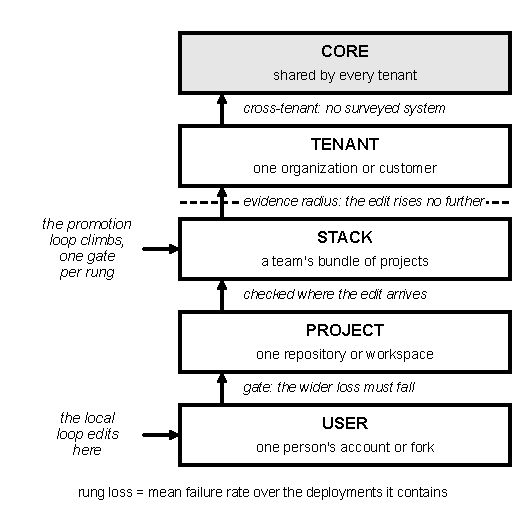
\includegraphics[width=\columnwidth]{fig2_scope_ieee}
\caption{Promotion scopes, from a user account to the shared core. Wider adoption changes the population on which an edit acts. Receiving-side evaluation checks whether the improvement is supported for the recipient.}
\label{fig:scope}
\end{figure}

A lower average loss at a broad scope can therefore conceal harm to an individual recipient. For this reason, the architecture proposed in Section~\ref{sec:gap} includes a held-out check at the receiving tenant. Versioning and access control govern whether an edit may be delivered and reversed; receiving-side evaluation tests whether the recipient should use it.

Several systems already evaluate transfers within one operator. ShareMem consolidates memories from one user for another and evaluates them in the receiving context \cite{hu2026sharemem}. XRepoSkill verifies a rule in at least two repositories \cite{guo2026xreposkill}. Evo2Team promotes routing skills between teams and confirms them at the target \cite{wang2026evo2team}.

Federated systems place the check at an aggregator or a server. EvolveNet checks at the aggregator, merging a shared harness only when the merge fixes at least as many held-out items as it breaks \cite{nie2026evolvenet}. FederatedSkill's server agent applies, adapts, or rejects each client's edit and records the decision \cite{yang2026federatedskill}. Their clients are partitions or agent instances under one operator, not independently governed customer organizations, so neither system instantiates a receiving-organization gate.

Where the check runs matters, and so does what it covers. Even in Evo2Team, nearly a fifth of confirmed transfers fail on graphs not covered by confirmation. A receiving-side check provides necessary evidence for adoption, but its finite cases do not guarantee performance on all future tasks.

\subsection{Automatic, human, and unchecked promotion}\label{automatic-human-and-unchecked-promotion}

Research systems often promote by admitting a candidate to a bank or archive that later runs draw on. SkillOpt, DGM, ADAS, Voyager, and SAGE make these admission decisions by program \cite{yang2026skillopt, zhang2025darwin, hu2024adas, wang2023voyager, wang2025sage}. AlphaEvolve and its predecessor FunSearch score candidates before admitting them to the archive \cite{alphaevolve2025, romeraparedes2024funsearch}. AlphaEvolve has produced gains used within Google, but it is a research loop within one operator, rather than a product for governed sharing between organizations. No candidate travels beyond the archive, and none of these systems has access control, audited promotion, or a gate at a receiving organization.

Automatic admissions differ in what they establish. NanoResearch merges semantically, AutoManual rewrites and consolidates by judgment, and ShareMem consolidates by judgment; each decision is programmatic, but none estimates a candidate's reduction in patch loss. The feedback classes anticipated this distinction: a program can decide promotion where no per-edit estimate of improvement exists.

Production systems more often retain a person at the promotion decision. Sierra routes generated insights through human-authored expert answers \cite{sierra2025os20}. In Devin, the same pull-request merge serves two roles: it supplies an observed outcome to local adaptation and records the reviewer's approval for the persistent repository \cite{cognition2025devinreview}. Spotify's optimized prompts and plans enter production after online A/B testing and a launch decision \cite{palumbo2026spotify}. CASCADE combines human and agent approval for memory consolidation \cite{huang2025cascade}. In each, the person at the promotion gate stands in for the exact signal production lacks. That substitution makes a program on the local gate with a person on the promotion gate the production-viable pairing rather than a compromise.

A None at the promotion gate has two meanings: sharing without a check, or no sharing at all. Letta's Context Repositories illustrate the first: background reflection writes local memory edits. In the released evidence, the only check on a local edit is an optional agent review before the edit is applied, and the edits then merge back automatically. That review is the basis for Letta's Auto local gate; with the option off, the system would sit in {[}None × None{]}. Letta then pushes shared-memory changes with git lineage but without an acceptance check, so the record explains what was shared without settling whether it should have been. AutoAgent illustrates the second, as do many other systems in which promotion is absent altogether: it revises the tool and peer descriptions of one agent without propagating those revisions to another deployment \cite{wang2026autoagent}.

\subsection{What formats, registries, and release platforms provide}\label{what-formats-registries-and-release-platforms-provide}

Much of the infrastructure needed for sharing already exists independently of these learning loops. Claude Agent Skills, Cursor Rules, GitHub Copilot instructions, Windsurf, Continue.dev, Zed, and Replit use git-tracked Markdown artifacts attached to workspaces, with a tool layer organized around MCP-style interfaces \cite{galster2026harnessconfig, barbaste2026harnessengineering}. This convergence makes artifacts easier to carry between runtimes. A study of repository-level loops nevertheless finds that the runtime state of the adaptation process remains outside version control \cite{lulla2026loopengineering}, so the portable file does not necessarily carry the history that produced it.

Public repositories provide a shared scope with human admission. In a study of five skill repositories, every substantive change was committed under a named human account and merged by a person; only one of 254 edits deprecated a skill \cite{shen2026whomaintains}. EDDOps gates promotion on evaluation thresholds before a human sign-off. MCP registries record namespaces and versions, and control planes add scanning, access control, or quarantine \cite{agenticcommunity2026mcpgateway, microsoft2026apicentermcp, truefoundry2026mcpgateway}. Governance registries add lineage and rollback \cite{kang2026registry, quessadavial2026acm, qin2026governed}; none of these registries generates candidate artifacts from failures.

Braintrust, Vellum, and LangSmith Hub likewise provide immutable versions, evaluation thresholds, and rollback \cite{braintrust2026docs, vellum2026docs, langsmith2026hub}. Engineers author the candidates, and evaluations can block a regressing release. In the surveyed descriptions, however, session feedback triggers neither candidate generation nor the release process, so these platforms supply much of the machinery for controlled change without closing the failure-driven local loop.

\subsection{The two decisions viewed together}\label{the-two-decisions-viewed-together}

Fig.~\ref{fig:design} places the local and promotion gates on a common grid, and Table~\ref{tab:VII-1} summarizes the occupants and their signals. The grid separates a system that generates and tests improvements from one that distributes human-authored artifacts under admission control, and it sets their complementary capabilities side by side.

\begin{figure}[!t]
\centering
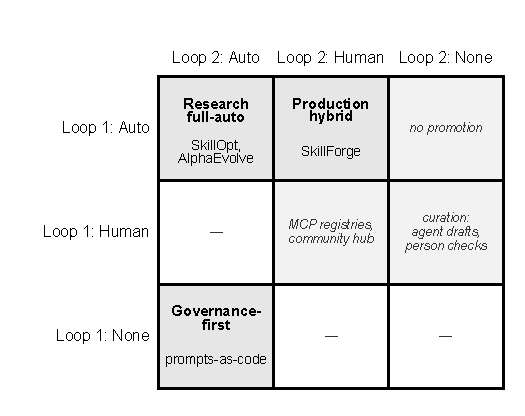
\includegraphics[width=0.95\columnwidth]{fig3_design_space_ieee}
\caption{Local and promotion gates. Each axis records who accepts a change: a program, a person, or no gate. None includes both absent promotion and unchecked sharing; the text distinguishes these cases.}
\label{fig:design}
\end{figure}

\begin{table*}[!t]
\caption{The gate grid read cell by cell: who keeps a local edit and who lets it climb, which systems sit in the cell, and the feedback signal they gate on. {[}Human × Auto{]} and {[}Human × Human{]} hold no surveyed system.}\label{tab:VII-1}
\centering\small
\begin{tabular}{@{}
  >{\raggedright\arraybackslash}p{(\textwidth - 6\tabcolsep) * \real{0.1613}}
  >{\raggedright\arraybackslash}p{(\textwidth - 6\tabcolsep) * \real{0.2903}}
  >{\raggedright\arraybackslash}p{(\textwidth - 6\tabcolsep) * \real{0.3065}}
  >{\raggedright\arraybackslash}p{(\textwidth - 6\tabcolsep) * \real{0.2419}}@{}}
\toprule\noalign{}
\begin{minipage}[b]{\linewidth}\raggedright
Cell
\end{minipage} & \begin{minipage}[b]{\linewidth}\raggedright
Who keeps the local edit, who lets it climb
\end{minipage} & \begin{minipage}[b]{\linewidth}\raggedright
Who is there
\end{minipage} & \begin{minipage}[b]{\linewidth}\raggedright
Signal found there
\end{minipage} \\
\midrule\noalign{}


{[}Auto × Auto{]} & A program keeps it; a program lets it climb & Research systems that close both halves inside one environment or one operator & Exact and simulated outcomes; delayed and judged only under pruning or merging \\ \addlinespace[2.5pt]
{[}Auto × Human{]} & A program keeps it; a person lets it climb & Production systems with a reviewer on promotion, and CASCADE & Observed outcomes and judgments \\ \addlinespace[2.5pt]
{[}Auto × None{]} & A program keeps it; nothing lets it climb & Letta's ungated push; systems that promote nothing & As on the local gate \\ \addlinespace[2.5pt]
{[}Human × None{]} & A person keeps it; nothing lets it climb & Curation & Judged \\ \addlinespace[2.5pt]
{[}None × Auto{]} & No failure triggers a candidate; a threshold gates release & Prompts-as-code platforms and governance registries & No failure-driven loop \\ \addlinespace[2.5pt]
{[}None × Human{]} & No failure triggers a candidate; a person admits & Open standards, MCP registries, community hubs & No failure-driven loop \\ \addlinespace[2.5pt]
{[}None × None{]} & Nothing checks or promotes the edit & SkillRL and SkillForge, unchecked skill loops & Outcomes and judgments \\ \addlinespace[2.5pt]
\bottomrule\noalign{}
\end{tabular}
\end{table*}
The occupied cells match the feedback-based expectations once automatic admission is distinguished from loss estimation. Where an {[}Auto × Auto{]} promotion gate estimates a loss change, the operative signals are exact checks or simulated outcomes; the cell's judged and delayed cases prune, rewrite, or merge instead. {[}Auto × Human{]} contains observed outcomes and judgments, with no exact-signal system in the surveyed cell.

The {[}Human × Auto{]} and {[}Human × Human{]} cells are empty in the surveyed set: no system combines a human local gate on a failure-driven loop with subsequent promotion. Human local decisions occur in curation.

The bottom row, where no local gate operates, holds two kinds of system. It holds comparison systems without a failure-driven local loop, such as prompt platforms, registries, and community hubs including Buildrix \cite{jiang2026buildrix}. SkillRL and SkillForge occupy {[}None × None{]} because neither checks its failure-driven skill updates: new skills in SkillRL, rewrites in SkillForge.

The audit's boundary cases leave the grid unchanged. Six systems promote without artifact lineage. Five, including Spotify, have sufficient evidence under the evidence-tier rule and enter already occupied cells when the audit is relaxed; the sixth, Future AGI's prompt lifecycle, has only uncorroborated T5 evidence. No relaxation yields governed promotion across organizations. Across the grid, capabilities divide: no system has both the learning of the top row and the governance of the bottom row.

\section{How adaptation can undermine its own evidence}\label{sec:failure}

Each edit the loop keeps or promotes changes the context of its next decision. New rules can conflict with old ones, a corrected memory can still be retrieved in its earlier form, and a frequently reused evaluator can become a target. These failures extend the technical-debt concerns that Sculley et al.~identified for machine-learning systems \cite{sculley2015debt}. Table~\ref{tab:X-1} pairs each failure with its control in the loop. The literature documents six of them in a measured case; the seventh, overfitting to one deployment, follows from the scope of the loss rather than from a measurement. Production systems provide the individual controls, but no surveyed system runs them together.

\begin{table*}[!t]
\caption{The failure surface of patchwork scaffold maintenance: what goes wrong, the piece of the loop that answers it, and the feedback-signal class in which it dominates.}\label{tab:X-1}
\centering\small
\begin{tabular}{@{}
  >{\raggedright\arraybackslash}p{(\textwidth - 6\tabcolsep) * \real{0.1463}}
  >{\raggedright\arraybackslash}p{(\textwidth - 6\tabcolsep) * \real{0.3659}}
  >{\raggedright\arraybackslash}p{(\textwidth - 6\tabcolsep) * \real{0.3659}}
  >{\raggedright\arraybackslash}p{(\textwidth - 6\tabcolsep) * \real{0.1220}}@{}}
\toprule\noalign{}
\begin{minipage}[b]{\linewidth}\raggedright
Failure
\end{minipage} & \begin{minipage}[b]{\linewidth}\raggedright
What goes wrong
\end{minipage} & \begin{minipage}[b]{\linewidth}\raggedright
The loop piece that answers it
\end{minipage} & \begin{minipage}[b]{\linewidth}\raggedright
Dominant class
\end{minipage} \\
\midrule\noalign{}


Scaffold bloat & Rules and skills accumulate until the model follows them worse and the gate has no clean signal & Complexity penalty \(\Omega\) in the gate; pruning and expiry as first-class gated operations & C1, C3 \\ \addlinespace[2.5pt]
Poisoned memory & An attacker writes an entry that later retrieval trusts & Provenance on every entry; write gating; a rollback envelope & C2 \\ \addlinespace[2.5pt]
Injection via tools and MCP & A tool's output or a connected server carries instructions into context & Narrow tool permissions; a privilege hierarchy over instructions; tool bindings pass the same promotion gate as any other coordinate & C2 \\ \addlinespace[2.5pt]
Evaluation fragility & The suite that gates edits is itself edited, gamed, and read non-independently & Held-out evaluations scoped within evidence radius, weighted toward recurring modes, re-read as the target drifts, checked against attribution & C3 (primary), C1 \\ \addlinespace[2.5pt]
Coordination failures & Multi-agent roles blur and context is lost between agents & Orchestration topology treated as a scaffold coordinate under the same gate and rollback discipline & C2 \\ \addlinespace[2.5pt]
Patch overfitting & A scaffold tuned to one deployment degrades another & Evidence-radius discipline at promotion; receiving-side held-out evaluation & C2 \\ \addlinespace[2.5pt]
Plasticity loss & Old rules, polluted memory, and drifting tool versions crowd out adaptation & Expiry and rollback as explicit loop operations rather than retrospective hygiene & C4 \\ \addlinespace[2.5pt]
\bottomrule\noalign{}
\end{tabular}
\end{table*}
\subsection{Accumulation and contamination}\label{accumulation-and-contamination}

Accumulated instructions become harder to follow and slow the response \cite{jaroslawicz2025ifscale}. At the system level, Ratchet finds that model-written skills need lifecycle hygiene before they produce gains \cite{zhang2026ratchet}. Conflicting or obsolete artifacts also complicate attribution: an evaluation may detect a failure without revealing whether the new candidate or an older artifact caused it. Gated retirement, pruning, and expiry preserve the conditions under which a new edit can be meaningfully assessed.

Persistent memory and connected tools create another route to lasting error. PoisonedRAG demonstrates attacks on retrieved knowledge \cite{zou2024poisonedrag}, AgentPoison plants backdoors in long-term memory or knowledge bases \cite{chen2024agentpoison}, and memory control-flow attacks operate across major agent frameworks \cite{xu2026mcfa}. Tool outputs and connected servers can insert instructions into the model's context \cite{greshake2023injection, debenedetti2024agentdojo}. In CVE-2025-54136, a previously approved MCP configuration could be changed without renewed approval \cite{checkpoint2025mcpoison}.

These failures motivate the memory controls \cite{su2026chronomem, yu2026rollbackrepair} and tool controls \cite{wallace2024hierarchy} listed in the table above, and also controlled revision of the tool binding itself. A check made only at the initial registration leaves later changes outside the decision that authorized the binding.

Rollback also needs to account for derivation: restoring a contaminated skill's earlier version does not remove the skills derived from it. VaG recovers little after such rollback \cite{shang2026vag}, which supports checking for contamination before commitment and tracking consequences afterward. A version history is a prerequisite for this tracking but does not by itself perform the recovery.

\subsection{When the evaluator changes}\label{sec:reflexive}

Consider a pitch-review assistant that consistently overrates decks claiming a large market without supporting numbers. The team revises its rubric from ``evaluate market size'' to ``require a numeric estimate and a source.'' The edit may improve reviews, but it also changes the standard used to evaluate subsequent behavior. If the same rubric judges future rubric revisions, the improvement process is modifying its own measuring instrument.

This is the reflexive-gate problem introduced with C3 feedback. Three scaffold systems (SkillForge, SkillChain, and SkillCoach) report calibrating a judge against people \cite{skillforge2026, hu2026skillchain, zhu2026skillcoach}, but no surveyed system reports calibration maintained across continuing rubric revisions and deployment drift. SkillCoach also evaluates its judge after editing it, in an offline audit that its authors describe as judge-assisted rather than a new human annotation study \cite{zhu2026skillcoach}. The audit compares the initial and evolved rubrics against human-gold references on 50 paired instances from 10 held-out task families, and trajectory-filtering consistency rises from 82\% to 96\%.

Weight-level reinforcement learning meets a related problem when it extends verifiable rewards to open-ended tasks; its methods, compared in the audit notes (Supplementary Material S6), are not included in the scaffold scores. Some hold the judge fixed, using checklists, pairwise preferences, references, or rubrics \cite{gunjal2025rubrics, jia2025writingzero, shi2026references, jin2026rlaes}. Others update the reward, rubric, or judge alongside the policy \cite{yu2025rlpr, xu2026rubricarm, ding2026evorubrics, zhu2026score, li2026rubricem}. Among the co-evolving methods reviewed, only RLPR reports agreement with human labels, and its reward is a probability rather than a rubric.

Even a fixed evaluator can become unreliable through repeated use. It remains subject to the proxy overoptimization \cite{gao2023overoptimization} and the shifting human criteria \cite{shankar2024validators} described for judged feedback, and unequal exposure to evaluation data can create apparent performance gains \cite{singh2025leaderboard}. Evaluations of agent trajectories are also path-dependent, and deployment tasks drift while the suite stays fixed. A gate therefore needs its own held-out checks, calibration where judgment is involved, and a revision history.

The hypothesis in Section~\ref{sec:why}, that failures in a bounded deployment fall into a catalogue of modes, has a conditional implication: if deployment failures concentrate in recurring modes, uniformly sampled tasks may underrepresent the modes that most need correction. Evaluation should then include those modes while preserving a held-out assessment. Score alone is not enough: it cannot tell a harness optimizer from trial and error \cite{ong2026harnesseval}, so the evaluation must also test the claimed link between failures and edits.

\subsection{Scope, coordination, and drift}\label{scope-coordination-and-drift}

Some failures arise from the structure of the deployment. Cemri et al.~identify fourteen failure modes in multi-agent systems, prominently including role confusion and context lost between agents \cite{cemri2025mast}. Treated as editable scaffold coordinates, routing and role assignments become subject to evaluation and rollback alongside instructions and skills.

Patch overfitting follows from specialization: a scaffold adapted to one deployment can degrade another, because the tasks and preferred behavior differ. Receiving-side evaluation limits this risk at promotion, and the evidence radius records where the improvement has been tested.

Finally, a scaffold can lose plasticity, becoming less adaptable as old and polluted artifacts accumulate. Long-context degradation \cite{liu2023lostmiddle} is one mechanism related to this loss. Expiry, pruning, and rollback must remain available throughout the system's lifetime, especially when delayed feedback arrives too slowly to keep the artifacts current.

No failure is exclusive to one feedback class, but the classes help organize the failure surface. Exact checks invite suite overfitting and cheap accumulation; observed outcomes depend on channels vulnerable to poisoning and injection; judged feedback is exposed to proxy optimization and moving criteria; delayed feedback makes drift difficult to correct promptly. Production systems provide individual controls, but the failure surface stays largely unmitigated because no surveyed system runs them together.

\section{What governed sharing would require}\label{sec:gap}

The evidence so far identifies a practical integration problem. Local optimizers can propose and test changes. Release platforms can version artifacts and reverse deployments. Registries can govern admission and access. The surveyed systems do not connect these capabilities into a process that learns in one organization and shares the resulting improvement with another under equivalent controls.

We audit that missing combination through four properties:

\begin{enumerate}
\def\labelenumi{(\alph{enumi})}
\tightlist
\item
  \textbf{An auto-gated local loop:} an algorithmic acceptance criterion tests a proposed artifact change.
\item
  \textbf{Cross-organization promotion:} artifacts can be promoted between independently governed organizations or customers.
\item
  \textbf{Versioned lineage with access control:} a promoted artifact carries its history and audit trail, and policies control who may access the artifact.
\item
  \textbf{Rollback:} a harmful promotion can be reversed without redeploying the whole system.
\end{enumerate}

In this audit, \emph{cross-tenant} and \emph{cross-organization} name the same boundary. Property (b) is not met by sharing among agents, users, or benchmark partitions within one operator.

Table~\ref{tab:IX-1} compares the closest systems, and each covers only part of the four properties. FederatedSkill \cite{yang2026federatedskill} and EvolveNet \cite{nie2026evolvenet} both adapt locally and share the result, but stay within one operator. Governance registries supply lineage and rollback without a local learning loop, and MCP control planes supply access control alone. Rollback exists inside one federated round and inside single deployments; no system rolls back a promotion that has crossed an organization boundary, because none makes such a promotion.

\begin{table*}[!t]
\caption{The closest approaches to governed cross-organization scaffold optimization, scored against the four properties.}\label{tab:IX-1}
\centering\small
\begin{tabular}{@{}
  >{\raggedright\arraybackslash}p{(\textwidth - 8\tabcolsep) * \real{0.1556}}
  >{\raggedright\arraybackslash}p{(\textwidth - 8\tabcolsep) * \real{0.2000}}
  >{\raggedright\arraybackslash}p{(\textwidth - 8\tabcolsep) * \real{0.2444}}
  >{\raggedright\arraybackslash}p{(\textwidth - 8\tabcolsep) * \real{0.2222}}
  >{\raggedright\arraybackslash}p{(\textwidth - 8\tabcolsep) * \real{0.1778}}@{}}
\toprule\noalign{}
\begin{minipage}[b]{\linewidth}\raggedright
System
\end{minipage} & \begin{minipage}[b]{\linewidth}\raggedright
(a) auto-gated local loop
\end{minipage} & \begin{minipage}[b]{\linewidth}\raggedright
(b) cross-organization promotion
\end{minipage} & \begin{minipage}[b]{\linewidth}\raggedright
(c) versioned lineage with access control
\end{minipage} & \begin{minipage}[b]{\linewidth}\raggedright
(d) rollback
\end{minipage} \\
\midrule\noalign{}


FederatedSkill \cite{yang2026federatedskill} & full & partial: privacy-preserving aggregation of skill edits across heterogeneous clients that sit under one operator & partial: auditable per-modification decision log & none \\ \addlinespace[2.5pt]
EvolveNet \cite{nie2026evolvenet} & full & partial: held-out merge gate at the aggregator, but clients are benchmark partitions, not organizations & none: no lineage, no access control & full: rollback to the previous shared harness after a failed round \\ \addlinespace[2.5pt]
SkillForge \cite{skillforge2026} & none: a calibrated judge selects the failures, nothing tests the rewrite & none: skill versions stay in the scenario deployment & partial & not documented \\ \addlinespace[2.5pt]
Governance-first registries \cite{kang2026registry, qin2026governed, quessadavial2026acm} & none: no inner loop & none & partial: lineage without access control & full, with evidence \\ \addlinespace[2.5pt]
MCP control planes \cite{agenticcommunity2026mcpgateway} & none: no inner loop & none & partial: access control without lineage & not reported \\ \addlinespace[2.5pt]
\bottomrule\noalign{}
\end{tabular}
\end{table*}
Receiving-side evaluation is an additional requirement on the promotion decision. We keep it separate from the four-property audit, which records loop, scope, and governance capabilities, because a system could have all of them and still decide without support whether an artifact benefits its recipient.

An architecture that addresses both would contain five connected parts: per-tenant artifact pools with provenance; an aggregation or selection process that respects tenant isolation; held-out evaluation at the receiving tenant; versioned lineage and access control; and a defined reversal path for each promoted artifact. The recipient's check would reject a promotion that does not lower its own patch loss. VaG's result (Section~\ref{sec:findings}) suggests that the reversal path would also need to track an artifact's descendants.

Federated learning offers a comparison, but the representation being shared is different. FedAvg combines comparable numeric updates, and its privacy and deployment problems have been extensively studied \cite{mcmahan2017fedavg, mcmahan2018dpfedavg, kairouz2021federated}. Federated prompt tuning moves the learned object to a shared prompt \cite{guo2022promptfl}. The nearest scaffold systems instead often use a language model to select, revise, or merge symbolic edits. Averaging is an appropriate analogy only where the artifact updates have a mergeable representation.

How far to automate should depend on the feedback. With exact checks, a transferred skill can be tested most directly, although the recipient still needs relevant test cases. Observed outcomes require evaluation on the recipient's workload because the sender's outcome is not portable evidence of success. For judged quality, a human promotion gate supported by lineage and rollback is a reasonable design choice. Delayed outcomes cannot support an immediate per-edit automatic local gate of the kind property (a) describes; systems with delayed outcomes still benefit from provenance and reversibility around proposals and milestones.

Thus the four properties define a target for the settings that can support an automatic local gate, not a requirement to automate every decision in every domain. The common requirement is that the evidence attached to an edit remain meaningful where the edit is used, and that the system still be able to inspect and reverse the edit's adoption.

\section{How the research lines fit together}\label{sec:families}

The loop is uneven because the research that built it started from different problems. Five research lines began with improving prompts, learning in context, selecting agent workflows, maintaining skill libraries, or transferring experience. Each developed the part of the loop most relevant to its starting problem, so the loop has grown from evaluation backward toward failure capture. Table~\ref{tab:VIII-1} places the lines side by side.

\begin{table*}[!t]
\caption{Five research lines converging on artifact-layer descent: the problem each started from, the part of the loop it built, and what it leaves open.}\label{tab:VIII-1}
\centering\small
\begin{tabular}{@{}
  >{\raggedright\arraybackslash}p{(\textwidth - 6\tabcolsep) * \real{0.1395}}
  >{\raggedright\arraybackslash}p{(\textwidth - 6\tabcolsep) * \real{0.2326}}
  >{\raggedright\arraybackslash}p{(\textwidth - 6\tabcolsep) * \real{0.3488}}
  >{\raggedright\arraybackslash}p{(\textwidth - 6\tabcolsep) * \real{0.2791}}@{}}
\toprule\noalign{}
\begin{minipage}[b]{\linewidth}\raggedright
Research line
\end{minipage} & \begin{minipage}[b]{\linewidth}\raggedright
Started from
\end{minipage} & \begin{minipage}[b]{\linewidth}\raggedright
The part of the loop it built
\end{minipage} & \begin{minipage}[b]{\linewidth}\raggedright
What it leaves open
\end{minipage} \\
\midrule\noalign{}


Reflective evolution & Prompt optimization and continual learning & Condition 4, the candidate: proposal by reflection over trajectory evidence; the two-timescale case for editing outside the weights & A persistent artifact; a bounded step; a held-out gate \\ \addlinespace[2.5pt]
Reflective context & Learning in context as a setting of its own & Condition 5, the penalty: the learned object in context space; a generalization penalty, the \(\Omega\) of the gate & A cross-deployment promotion loop \\ \addlinespace[2.5pt]
Harness optimization & Orchestration and harness engineering & Condition 3, the trace: attribution of a failure to one slot of the orchestration graph; source-level edits & Attribution across substrates; a governed promotion loop; access control; rollback \\ \addlinespace[2.5pt]
Lifecycle and multi-objective & Skill pools that bloat under platform limits & The gate on removal: gated retirement; hygiene as a precondition; a hard frontier as the shape of \(\Omega\) & Closing the loop as descent; retiring a promoted artifact's descendants \\ \addlinespace[2.5pt]
Transfer and federation & How far an edit travels & The promotion loop, the check on arrival: evidence radius measured one task at a time; cross-client aggregation; receiving-side confirmation & A cross-organization gate, lineage, and rollback \\ \addlinespace[2.5pt]
\bottomrule\noalign{}
\end{tabular}
\end{table*}
The first three lines each built one condition. Prompt optimization and reflective evolution developed ways to propose edits from trajectory evidence, with an argument for adapting artifacts on a faster schedule than weights \cite{agrawal2025gepa, tiwari2026fastandslow}. Reflective Context Learning formalizes learning in context and the need to control generalization, which corresponds to the complexity penalty in the acceptance rule \cite{vassilyev2026rcl}. Harness optimization treats source-level orchestration changes as the learned object and repeatedly identifies attribution as its difficult step \cite{lee2026metaharness, lin2026ahe, cai2026moss, zehle2026cantante, nguyen2026harnessevo, chen2026harnessforge, li2026growingharness}.

The last two lines study artifacts after they are kept. The lifecycle literature starts from skill pools that can become too large or internally inconsistent to remain useful; its work includes evaluated retirement, hygiene, and optimization under platform limits \cite{zhang2026ratchet, tanjim2026mocha, liu2026skillsvote, zhang2026librarydrift, wei2026skillsmith, pu2026skillops, wang2026assay}. Transfer and federation ask how far a learned artifact remains useful, progressing from cross-task measurements to receiving-team confirmation and shared client updates \cite{shalev2026ict, li2026combee, qu2026coral, ling2026pace, wang2026evo2team, yang2026federatedskill, nie2026evolvenet}.

This history helps explain why evaluation and proposal mechanisms are more developed than failure capture. Each research line inherits its loss from its benchmark and begins with available trajectories. None began by recording recurring failures. Attribution receives substantial attention, but usually within each line's own substrate. The local loop has consequently developed from evaluation backward toward the evidence needed to choose a useful edit.

The five lines converge: different starting problems repeatedly lead to comparable mechanisms for proposing, testing, retaining, and reusing changes. The convergence does not establish that one architecture is optimal, and none of these lines documents the complete cross-organization process, but it supports a shared decomposition of the system into weights and editable artifacts. GEPA, Meta-Harness, MOSS, RCL, PACE, and the harness-optimization papers all use that decomposition; SIA updates both and still treats them as separate levers \cite{hebbar2026sia}.

\subsection{Why specialization remains outside the weights}\label{sec:why}

A general model and a particular deployment face different requirements. The model must work across many settings. A deployment must follow its own conventions, honor its users' preferences, and avoid failures that may be rare globally but frequent locally. The scaffold encodes those requirements at a scope narrower than the model's entire user population.

Two lines of work help motivate the distinction between broad model behavior and customer-specific requirements. Studies of reinforcement learning from human feedback report reduced output diversity and more homogeneous preferences \cite{kirk2024understanding, padmakumar2023diversity}. Tiwari et al.~approach the distinction from adaptation cost: in-context changes are cheap but capacity-bounded, while in-weight adaptation is more expressive and can introduce forgetting and loss of plasticity \cite{tiwari2026fastandslow, dohare2024loss}.

Per-customer adapters \cite{hu2021lora}, distilled models, and learned routing can absorb some local requirements. They also introduce separate training, evaluation, and serving lifecycles. Persistent artifacts offer the cheaper path: they are inspectable, reversible, scoped to one customer, and updatable daily.

Two earlier papers in this series offer a hypothesis for why targeted artifact changes may be effective. \emph{Beyond Exponential Decay} argues that long-output reliability depends on a sparse set of key decisions rather than a uniform error probability at every token \cite{arbuzov2025beyond}. Its evidence includes the accuracy recovered through majority voting on reasoning benchmarks and long-range dependence measured on one natural-text corpus, where fewer than a tenth of tokens depend on distant context. Its argument is limited when the number of consequential decisions grows with the task, as in long-horizon agentic work.

\emph{The Architecture of Errors} considers a bounded deployment with recurring tasks, tools, and evaluator expectations \cite{arbuzov2026architecture}. It argues that failures there fall into a catalogue of modes whose size grows slowly with observed experience. Under its assumptions, the intervention budget grows polylogarithmically with sequence length and becomes constant once the catalogue saturates. It also gives a negative result: a finite catalogue cannot cover an unbounded domain.

If these hypotheses generalize, a deployment may be improved through a manageable set of targeted interventions. Persistent rules, memories, skills, and tool changes represent those interventions in inspectable form. On that hypothesis the gated and scoped artifact layer is not a workaround for an inadequate model but the architecture the error structure calls for: a frontier model that generalizes, a local scaffold that specializes, and reliability that comes from governing the specialization. The survey does not test the hypotheses: its findings about acceptance gates, feedback, and promotion rest on the corpus alone.

\subsection{Relation to neighboring surveys}\label{relation-to-neighboring-surveys}

Existing surveys organize the field around agent evolution, persistent state, context engineering, skills, memory security, and harness design. This survey follows a different unit of analysis: the decision that accepts a persistent change, the feedback supporting that decision, and the scope in which the change is then used. Table~\ref{tab:II-2} records the distinction for each neighboring survey.

\begin{table*}[!t]
\caption{Neighboring surveys and where this one departs from each. This survey classifies by loop closure, gate type, signal class, and governance, and is the only one to cover promotion across organizations.}\label{tab:II-2}
\centering\small
\begin{tabular}{@{}
  >{\raggedright\arraybackslash}p{(\textwidth - 4\tabcolsep) * \real{0.1757}}
  >{\raggedright\arraybackslash}p{(\textwidth - 4\tabcolsep) * \real{0.2027}}
  >{\raggedright\arraybackslash}p{(\textwidth - 4\tabcolsep) * \real{0.6216}}@{}}
\toprule\noalign{}
\begin{minipage}[b]{\linewidth}\raggedright
Survey
\end{minipage} & \begin{minipage}[b]{\linewidth}\raggedright
Scope
\end{minipage} & \begin{minipage}[b]{\linewidth}\raggedright
How this survey differs
\end{minipage} \\
\midrule\noalign{}


Gao et al. \cite{gao2026selfevolving} & self-evolving agents & organizes by what, when, how, and where an agent evolves; the gate that accepts an edit, and the edit's scope, are mentioned but not classified \\ \addlinespace[2.5pt]
Fang et al. \cite{fang2025comprehensive} & self-evolving agents & organizes by inputs, agent system, environment, and optimizer; loop closure appears in passing, gates and promotion do not \\ \addlinespace[2.5pt]
Zhou et al. \cite{zhou2026selfevolvingcoding} & self-evolving coding agents (108 methods) & organizes by evolution target, timing, and code signal; closest on reversibility, with no gate or promotion axis \\ \addlinespace[2.5pt]
Ding et al. \cite{ding2026alwayson} & persistent-state agents (435 works) & organizes by authority, scope, mutability, provenance, and recoverability of state; governance is an axis, the gate on an edit is not \\ \addlinespace[2.5pt]
Lin et al. \cite{lin2026memorysecurity} & memory security (\textasciitilde90 works) & organizes by lifecycle phase and security objective; principal scoping and rollback are axes, feedback and promotion are not \\ \addlinespace[2.5pt]
Guo et al. \cite{guo2026harness} & agent system and harness design & organizes by six runtime responsibilities; touches all four questions without classifying by any \\ \addlinespace[2.5pt]
Xia et al. \cite{xia2026harnessing} & skill-mediated agents (8 systems) & organizes by four responsibility layers and ten patterns; loop closure and governance appear as patterns, not as axes \\ \addlinespace[2.5pt]
Ding et al. \cite{ding2026skilleval} & skill evaluation and evolution & organizes by four evolution paradigms and six benchmark classes; evaluation is the subject, the gate it feeds is not \\ \addlinespace[2.5pt]
Mei et al. \cite{mei2025context} & context engineering (1,411 papers) & organizes by components and system implementations; adaptation loops lie outside its scope \\ \addlinespace[2.5pt]
\bottomrule\noalign{}
\end{tabular}
\end{table*}
The closest governance precedents are Ding et al.'s survey of persistent-state agents and Lin et al.'s memory-security survey \cite{ding2026alwayson, lin2026memorysecurity}. The persistent-state survey finds greater attention to accumulating and retrieving state than to governing, recovering, or relinquishing it. The memory-security survey treats scoping and rollback as security primitives. Neither asks who gates an edit, and neither covers promotion across organizations.

Optimizers of prompts, where the first research line started, and of programs and scaffolds establish many of the underlying mechanisms. OPRO, EvoPrompt, Promptbreeder, DSPy, and TextGrad optimize a prompt or program once against development evidence and are not deployed loops \cite{yang2023opro, guo2023evoprompt, fernando2023promptbreeder, khattab2023dspy, yuksekgonul2024textgrad}. ACE persists an evolving playbook but never promotes it \cite{ace2025agentic}. Agent symbolic learning treats prompts, tools, and pipelines as symbolic parameters \cite{zhou2024symbolic}; STOP improves its own scaffolding program \cite{zelikman2023stop}; and SICA edits its harness to improve benchmark performance \cite{robeyns2025sica}.

The survey's contribution is to read these precedents jointly at deployment scope: whether an artifact persists, whether a local acceptance decision is made, which signal supports it, and what authorizes use elsewhere. Its 256-system corpus, two-loop classification, feedback classes, and governance audit, which an extended discussion separates from their precedents (Supplementary Material S7), make that joint reading explicit.

\section{Open problems and conclusion}\label{sec:open}

Five problems remain, each sharper when stated as a decision a deployment must make.

\textbf{Attributing a failure to an editable cause.} No surveyed method attributes a failure to the responsible instruction, memory, skill, or tool binding across all substrates, even where an exact check establishes that the output failed. Three methods provide narrower starting points: slot attribution \cite{nguyen2026harnessevo}, intervention-based attribution \cite{chu2026agentgrad}, and contrastive multi-agent attribution \cite{zehle2026cantante}. Attribution is harder under observed outcomes, whose causes are more confounded.

\textbf{Establishing improvement at the recipient.} A transferred artifact must be evaluated against the receiving deployment's tasks and measure. Receiving-side checks show that this evaluation is feasible in selected settings, and Evo2Team's failures on unseen graphs show the limits of the checks' coverage. Federated Agent Optimization proposes but does not implement a receiving-client gate \cite{yang2026fao}. Connecting such checks to provenance, access control, and reversal remains the architectural problem taken up last.

\textbf{Maintaining calibration while the criterion changes.} On judged tasks, a judge must stay aligned with people across continuing revisions of its rubric. SkillCoach shows that an evolved rubric can be audited offline against human-gold references \cite{zhu2026skillcoach}, but no surveyed scaffold system reports calibration maintained through repeated revisions in deployment. The neighboring reward literature also reports no human-agreement result for a co-evolving rubric or judge; RLPR's probability-based reward is a distinct case. A useful solution must evaluate the moving criterion as well as the outputs it scores.

\textbf{Evaluating improvement with delayed outcomes.} When many edits occur before a meaningful result arrives, no gate can accept each edit as it is made. Proxy milestones and proposal pruning may still be useful, but downstream gains alone do not establish successful attribution. Harness optimizers should therefore be assessed against both their final scores and their claims about why particular edits help \cite{ong2026harnesseval}.

\textbf{Connecting local learning to governed sharing.} No surveyed system combines automatic local acceptance, promotion across organizations, versioned lineage with access control, and rollback, although the components exist in different systems. A system that integrates them must preserve tenant isolation, evaluate the recipient, and account for artifacts derived from a change that is later withdrawn. Where feedback cannot support automatic acceptance, such a system must retain the corresponding human decision or delayed evaluation.

The survey's central observation is that persistent changes outside the weights have become an important form of adaptation, while the evidence supporting those changes remains fragmented. Many systems can test a local candidate. Fewer can reliably explain which recurring failure it addresses. None of the public systems examined here has assembled the machinery for transferring the resulting improvement to another organization.

The frontier model generalizes. The local scaffold specializes. Reliability comes from governing that specialization: knowing what each change improved, where that evidence applies, and how the change can be reversed. Such governance must extend to the evaluations themselves when they become part of the adapting system.

\section{Appendix: Formal statement of artifact-layer descent}\label{app:formal}

This appendix states the setup behind Section~\ref{sec:loop}, a one-step descent inequality under a noisy gate, an informal convergence statement, the optimization-analogy correspondence, and four worked cases. We claim no new theorem; the convergence statement is the ordinary target of local stochastic optimization under noisy estimators, restated for a discrete, versioned parameter.

\begin{table*}[!t]
\caption{Optimization concepts and their scaffold analogues.}\label{tab:A-1}
\centering\small
\begin{tabular}{@{}
  >{\raggedright\arraybackslash}p{(\textwidth - 2\tabcolsep) * \real{0.2333}}
  >{\raggedright\arraybackslash}p{(\textwidth - 2\tabcolsep) * \real{0.7667}}@{}}
\toprule\noalign{}
\begin{minipage}[b]{\linewidth}\raggedright
Optimization concept
\end{minipage} & \begin{minipage}[b]{\linewidth}\raggedright
Scaffold analogue
\end{minipage} \\
\midrule\noalign{}


Parameter vector & Instructions, skills, memories, tools, routing graphs, and governance rules, evaluation gates among them \\ \addlinespace[2.5pt]
Loss & Failure, user correction, evaluation regression, retrieval miss, tool error, schema violation \\ \addlinespace[2.5pt]
Gradient estimate & Credit assignment identifying the coordinate responsible for a failure \\ \addlinespace[2.5pt]
Step & Accepted scaffold edit; step size is edit magnitude under \(\oplus\) \\ \addlinespace[2.5pt]
Aggregated update & Several recurring failures combined before an update, by averaging or by agreement across \(k\) proposals \\ \addlinespace[2.5pt]
Update radius & Promotion scope: which loss is descended (USER, PROJECT, STACK, TENANT, CORE) \\ \addlinespace[2.5pt]
Validation loss & Held-out patch evaluation before merge \\ \addlinespace[2.5pt]
Regularization & Complexity penalty \(\Omega(z)\), bloat control, cross-patch regression checks \\ \addlinespace[2.5pt]
Overfitting & Scaffold improves on this deployment and degrades elsewhere \\ \addlinespace[2.5pt]
Rollback & Reverting a harmful accepted update \\ \addlinespace[2.5pt]
\bottomrule\noalign{}
\end{tabular}
\end{table*}
\subsection{Setup}\label{setup}

Let the frontier model have fixed parameters \(\theta_M\) and let the scaffold be a structured object \(\theta_s \in \Theta_s = \Theta_1 \times \cdots \times \Theta_6\) over the six substrate coordinates of Section~\ref{sec:method}; \(\Theta_s\) is discrete, symbolic, and versioned. For a deployment \(D\), \(L_D(\theta_s) = \mathbb{E}_{x \sim D}[\ell(\pi(\theta_M, \theta_s, x))]\). A candidate edit is drawn from a proposal process conditioned on the accumulated history \(H_t\) of failures, corrections, rejected outputs, evaluation regressions, and prior accepted edits: \(z_t \sim Q_t(z \mid H_t, \theta_s^t)\). \(Q_t\) is not uniform. A mode \(m\) that recurs with frequency \(f_m\) and carries per-occurrence loss \(s_m\) has expected contribution \(f_m s_m\) to the failure rate, so high-frequency or high-severity modes are proposed first. The finite directional difference is \(\Delta_z L_D(\theta_s) = L_D(\theta_s \oplus z) - L_D(\theta_s)\); the gate sees only a noisy estimate \(\widehat{\Delta}_z L_D\). The update is \[\theta_s^{t+1} = \theta_s^t \oplus z_t \text{ if } G_t(z_t) = 1, \quad \theta_s^{t+1} = \theta_s^t \text{ otherwise.}\]

\subsection{Descent inequality}\label{descent-inequality}

Per-step expected improvement is the gate's margin minus its estimator bias, weighted by acceptance probability. Write \(\mathcal{F}_t\) for the history up to step \(t\): the failures, corrections, edits, and gate decisions in \(H_t\) together with \(\theta_s^t\). Because the proposal \(Q_t\) depends on the whole history and not on \(\theta_s^t\) alone, every expectation and probability below conditions on \(\mathcal{F}_t\). Assume (A1) positive descent bias on accepted edits, \(\mathbb{E}[\widehat{\Delta}_{z_t} L_D \mid G_t = 1, \mathcal{F}_t] \le -\gamma_t - \tau_t\) for some \(\gamma_t > 0\), and (A2) bounded estimator bias on accepted edits, \(|\mathbb{E}[\Delta_{z_t} L_D - \widehat{\Delta}_{z_t} L_D \mid G_t = 1, \mathcal{F}_t]| \le \varepsilon_t\). With \(p_t = \Pr(G_t = 1 \mid \mathcal{F}_t)\), \[\mathbb{E}[L_D(\theta_s^{t+1}) \mid \mathcal{F}_t] \le L_D(\theta_s^t) - p_t(\gamma_t + \tau_t) + p_t\,\varepsilon_t.\] In the feedback-signal classes of Section~\ref{sec:signal}, \(\varepsilon_t\) is near zero for an exact check (C1), though the sampling error of a finite suite over the patch remains; bounded by batching for an observed outcome (C2); equal to the judge's bias, and bounded only by calibration, for a judged signal (C3); and unavailable per edit for a delayed signal (C4).

\subsection{Convergence (informal)}\label{convergence-informal}

Nothing in the survey depends on the convergence statement below. It holds under strong assumptions and is included to make gate stability precise. Add three assumptions. (A3) Proposal coverage with acceptance: at every non-gate-stable scaffold, \(Q_t\) places probability at least \(q > 0\) on an admissible edit with \(\mathbb{E}[\Delta_z L_D] \le -\delta\), and the gate accepts such an edit with probability at least \(q' > 0\), so that \(p_t(\gamma_t + \tau_t) \ge q q' \delta\) there. (A4) Effective compactness of the reachable orbit. (A5) Summable bias, \(\sum_t p_t \varepsilon_t < \infty\). Let \(0 \le L_D \le B\). (A3) is strong: it asks for a uniform lower bound on proposing and accepting an edit that lowers the loss by at least \(\delta\).

The one-step inequality is then of the Robbins--Siegmund form, a non-negative process that decreases in expectation up to a summable perturbation \(p_t \varepsilon_t\), so \(L_D(\theta_s^t)\) converges almost surely and \(\sum_t p_t(\gamma_t + \tau_t) < \infty\) almost surely \cite{robbins1971convergence}.

The content lies in the finite sum. A bounded loss cannot pay for infinitely many accepted edits with a positive expected margin, so under (A3) the process visits non-gate-stable scaffolds only finitely often. With (A4), the limit set of \(\{\theta_s^t\}\) is gate-stable, meaning that no admissible edit clears the gate with negative expected directional loss in the limit.

The result is convergence of the loss and stability of the gate decision, not convergence to an optimum. A globally suboptimal gate-stable scaffold is consistent with it, because \(Q_t\) may never propose the improving edit or \(\widehat{\Delta}\) may be biased to reject it.

The argument does not cover a non-stationary deployment (\(D = D_t\)). Tracking a moving optimum would need further assumptions, not supplied here, on the rate of drift and of adaptation. For that case, recency weighting, pruning, expiry, and rollback are the scaffold-level analogues of the machinery used in continual learning.

\subsection{Correspondence}\label{correspondence}

Table~\ref{tab:A-1} pairs each optimization concept with its scaffold analogue. Credit assignment here is attribution, not backpropagation: scaffold systems do not differentiate through instruction files but trace an output error to an upstream coordinate, manually or with a judge or verifier. The two formal results ask different things of that attribution. The one-step inequality needs only that accepted edits have positive expected descent. The convergence statement needs attribution reliable enough to supply the uniformly improving proposals that (A3) assumes. That requirement is much stronger than the credit-assignment condition of Section~\ref{sec:loop}, success with non-zero probability per failure.

\subsection{Worked cases}\label{worked-cases}

\emph{Retrieval.} Failures recur because retrieved context omits the decisive clause. Attribution traces the error to the retrieval coordinate: chunking, query rewriting, metadata filter, embedding model, reranker, or context-packing rule. The candidate edit tightens chunk boundaries or adds a metadata constraint, and the gate checks that recall and answer accuracy improve on the patch evaluation without degrading adjacent cases. Class C1 or C2.

\emph{Pitch review.} The system repeatedly overrates decks that claim a large market without numbers, and the failure cluster points at an under-specified rubric coordinate. The edit changes ``evaluate market size'' into ``require a numeric estimate and a source; if absent, cap the score''; the gate runs the revised rubric against held-out decks with human scores. What the edit changes is the gate that will judge the next edit: the reflexive gate of Section~\ref{sec:signal}. Class C3.

\emph{Tool use.} Calls fail because optional parameters are under-specified. The responsible coordinate may be the tool schema, the call policy, or the clarification rule. The edit adds required fields or a pre-call uncertainty check; the gate checks that tool-call failures fall without raising refusals or latency. Class C2.

\emph{Memory.} A stale customer preference is repeatedly retrieved and causes bad decisions. The responsible coordinate is a memory entry together with its provenance, priority, and expiry policy. The edit corrects, expires, or version-tags the entry; the gate checks that future behavior improves without erasing useful history. Class C2, with the correction itself observable only through a later outcome.

\section{Appendix: Gate families and feedback-signal classes}\label{app:gates}

Section~\ref{sec:loop} collapses every production gate into one per-edit test \(G_t\) on an estimate of the loss change. Surveyed systems instantiate that test in several ways. Some of these instantiations precede the per-edit gate and are better read as proposal pruning than as estimators of \(\widehat{\Delta} L_D\). Table~\ref{tab:B-1} lists the families, the slot each occupies, representative systems, and the feedback-signal class (Section~\ref{sec:signal}) each family serves.

\begin{table*}[!t]
\caption{Gate families, their slot in the formalism, and the feedback-signal class each serves.}\label{tab:B-1}
\centering\small
\begin{tabular}{@{}
  >{\raggedright\arraybackslash}p{(\textwidth - 8\tabcolsep) * \real{0.1463}}
  >{\raggedright\arraybackslash}p{(\textwidth - 8\tabcolsep) * \real{0.2683}}
  >{\raggedright\arraybackslash}p{(\textwidth - 8\tabcolsep) * \real{0.1707}}
  >{\raggedright\arraybackslash}p{(\textwidth - 8\tabcolsep) * \real{0.1707}}
  >{\raggedright\arraybackslash}p{(\textwidth - 8\tabcolsep) * \real{0.2439}}@{}}
\toprule\noalign{}
\begin{minipage}[b]{\linewidth}\raggedright
Gate family
\end{minipage} & \begin{minipage}[b]{\linewidth}\raggedright
What it estimates
\end{minipage} & \begin{minipage}[b]{\linewidth}\raggedright
Slot in Section~\ref{sec:loop}
\end{minipage} & \begin{minipage}[b]{\linewidth}\raggedright
Signal class
\end{minipage} & \begin{minipage}[b]{\linewidth}\raggedright
Representative systems
\end{minipage} \\
\midrule\noalign{}


Surrogate verifier & Pass or fail from tests, a symbolic checker, or an exact match & Per-edit gate \(G_t\) & C1 & DGM (sandboxed compile-and-edit check; score weights selection, not retention), SkillOpt (held-out exact match), Voyager (game-state check: C2) \\ \addlinespace[2.5pt]
Evaluation cascade & \(\widehat{\Delta} L_D\) on a held-out task suite, cheap-to-expensive evaluators & Per-edit gate \(G_t\) & C1 when the suite is exact; C2 when it is a task suite & AlphaEvolve, Braintrust, Vellum, LangSmith Hub \\ \addlinespace[2.5pt]
RL threshold & Reward improvement against a deployment threshold & Per-edit gate \(G_t\) & C2 & SAGE, PACE \\ \addlinespace[2.5pt]
LLM judge with calibration & Pairwise or rubric score, calibrated against human agreement & Per-edit gate \(G_t\) & C3 & SkillChain (judge stage, before its human reflection gate) \\ \addlinespace[2.5pt]
Reviewer judgment & Human credit assignment by pull-request review, expert sign-off, or a user's acceptance & Per-edit gate \(G_t\), human-instantiated & C3 (and C2 when the reviewer has outcome data) & Sierra Agent OS 2.0, Anthropic skills repository, CASCADE (a person and an agent approve consolidation into shared memory) \\ \addlinespace[2.5pt]
Semantic merge & Whether a candidate duplicates or conflicts with existing artifacts & Proposal pruning before \(G_t\) & C4 (also a pre-filter in C2, C3) & NanoResearch orchestrator, FederatedSkill server agent, EvolveR (admission: cosine pre-filter plus LLM equivalence judgment on each distilled principle; retention: periodic pruning on per-principle success rate) \\ \addlinespace[2.5pt]
Archive selection & Whether a candidate improves on, or diversifies, an archive of already-scored programs & Proposal pruning before \(G_t\) & Any; inherits the class of the evaluator that scored the archive (C1 in AlphaEvolve) & AlphaEvolve (MAP-Elites-style database), ADAS \\ \addlinespace[2.5pt]
Multi-sample agreement & Whether \(k\) independent proposals or evaluations agree; false-accept rate decays as \(p^k\) rather than variance as \(1/k\) & Aggregation filter on the estimate & C2, C3 noise absorption & VaG (three heterogeneous critics must all pass); SkillOpt-Lite (consensus filter across rollouts) \\ \addlinespace[2.5pt]
\bottomrule\noalign{}
\end{tabular}
\end{table*}
The first five families populate \(G_t\) directly and, under the assumptions of Appendix~\ref{app:formal}, inherit its descent guarantee. Semantic merge and archive selection, which are not estimators of \(\widehat{\Delta} L_D\), constrain the proposal distribution instead, and the descent argument applies to the composition of pruning and gate. Multi-sample agreement is the correct analogue of ``wait for \(k\) pieces of evidence before accepting an edit'', an operation distinct from, and not to be conflated with, mini-batch averaging.

Read down the signal-class column for the structural content of Section~\ref{sec:signal}. A judged (C3) deployment can use only the two families whose estimator is a judge. A delayed (C4) deployment has no family that estimates the loss change per edit. It has semantic merge before the gate and whatever proxy milestone stands at the horizon.


\section*{Acknowledgment}
% TODO(AI disclosure): IEEE Access requires disclosure of AI-generated text in the acknowledgments. Draft wording for the authors to approve:
The authors used an AI assistant (Claude, Anthropic) to help search the literature, check citations, and edit prose; all claims, scores, and classifications were reviewed and approved by the authors. Earlier versions of this argument appeared as an arXiv preprint and as a non-archival workshop submission; this article extends them with the feedback-signal classification of Section~IV and a corpus scored through October 2026.

\bibliographystyle{IEEEtran}
\bibliography{references}

% TODO(bios): biographies (100-150 words) and photos for all six authors.
\begin{IEEEbiographynophoto}{Mikhail L. Arbuzov}
TODO(bio).
\end{IEEEbiographynophoto}

\begin{IEEEbiographynophoto}{Lee Mosbacker}
TODO(bio).
\end{IEEEbiographynophoto}

\begin{IEEEbiographynophoto}{Sisong Bei}
TODO(bio).
\end{IEEEbiographynophoto}

\begin{IEEEbiographynophoto}{Ziwei Dong}
TODO(bio).
\end{IEEEbiographynophoto}

\begin{IEEEbiographynophoto}{Dmitri Kalaev}
TODO(bio).
\end{IEEEbiographynophoto}

\begin{IEEEbiographynophoto}{Alexey Shvets}
TODO(bio).
\end{IEEEbiographynophoto}

\EOD

\end{document}
